\documentclass[review]{elsarticle}

\usepackage{lineno,hyperref}
\modulolinenumbers[5]

\journal{Ocean Engineering }

%%%%%%%%%%%%%%%%%%%%%%%
%% Elsevier bibliography styles
%%%%%%%%%%%%%%%%%%%%%%%
%% To change the style, put a % in front of the second line of the current style and
%% remove the % from the second line of the style you would like to use.
%%%%%%%%%%%%%%%%%%%%%%%

%% Numbered
%\bibliographystyle{model1-num-names}

%% Numbered without titles
%\bibliographystyle{model1a-num-names}

%% Harvard
%\bibliographystyle{model2-names.bst}\biboptions{authoryear}

%% Vancouver numbered
%\usepackage{numcompress}\bibliographystyle{model3-num-names}

%% Vancouver name/year
%\usepackage{numcompress}\bibliographystyle{model4-names}\biboptions{authoryear}

%% APA style
%\bibliographystyle{model5-names}\biboptions{authoryear}

%% AMA style
%\usepackage{numcompress}\bibliographystyle{model6-num-names}

%% `Elsevier LaTeX' style
\bibliographystyle{elsarticle-num}
%%%%%%%%%%%%%%%%%%%%%%%

\begin{document}

\begin{frontmatter}

\title{Quantitative benchmark of a single rising bubble using VoF methods}

%% Group authors per affiliation:
\author[ifpenaddress]{Lionel Gamet\corref{mycorrespondingauthor}}
\cortext[mycorrespondingauthor]{Corresponding author}
\ead{Lionel.Gamet@ifpen.fr}
\ead[url]{www.ifpenergiesnouvelles.fr}

%% or include affiliations in footnotes:
\author[ifpenaddress]{Marco Scala}

\author[stromningaddress]{Johan Roenby}

\author[dlraddress]{Henning Scheufler}

\author[ifpenaddress]{Jean-Lou Pierson}

\address[ifpenaddress]{IFPEN Lyon, Process Experimentation Division, 69360 Solaize, France}
\address[stromningaddress]{STROMNING, Luftmarinegade 62, 1432 K{\o}benhavn K, Denmark}
\address[dlraddress]{DLR German Aerospace Center, Institute of Space Systems, 28359 Bremen, Germany}

\begin{abstract}
Free surfaces and fluid interfaces are encountered in a wide variety of gas-liquid configurations. Although many numerical approaches exist to solve such multiphase flows, there is still a need for improved simulation methods due to an increasing demand of highly resolved gas-liquid simulations. Recently, a new efficient geometric Volume of Fluid (VoF) method for general meshes, called isoAdvector, was published. More recently, a novel computational interface reconstruction scheme based on calculation of a reconstructed distance function (RDF) has been introduced. This new scheme has been combined with the interface advection step of the isoAdvector algorithm. Both methods have been implemented in the OpenFOAM Computational Fluid Dynamics (CFD) Open Source software package. Before running into complex tridimensional geometries, elementary quantitative benchmark configurations are essential for validation and comparison of interfacial flow solvers. Following the benchmark of Hysing, we present in this paper two quantitative benchmark configurations that we have used for validation and comparison of the isoAdvector interface reconstruction methods. Comparisons are conducted against literature reference data and also against the OpenFOAM VoF historical solver, \verb+interFoam+, solver employing the MULES limiter (Multidimensional Universal Limiter with Explicit Solution). The first validation case is a 2D single bubble rising in a quiescent liquid. Comparisons are presented using either hexahedral or triangular-prismatic grids. The RDF reconstruction method demonstrates a better behaviour, particularly on triangular grids. The second validation case is a 2D stagnant single bubble in a quiescent liquid, under zero gravity conditions. This second validation case has been derived from the first case in the objective of quantification of the spurious currents generated by the different VoF solvers employed in this study. The RDF reconstruction method demonstrates a strong reduction of the amplitude of spurious currents and a better prediction of the pressure jump across the bubble. 


\end{abstract}

\begin{keyword}
CFD \sep Multiphase flows\sep Bubbly flows\sep Incompressible\sep MULES\sep isoAdvector\sep Volume of Fluid \sep OpenFOAM\sep Spurious currents
\end{keyword}

\end{frontmatter}

\linenumbers

%%======================================================================
\section{Introduction}
%%======================================================================

Gas-liquid interfacial flow systems are often encountered in a wide variety of configurations, in science, engineering or industry. In ocean engineering, floating wind turbines, oil and gas platforms, or more generally coastal and offshore structures are submitted to violent waves, which is a paramount concern for their correct dimensioning. In the chemical process industry, various scales of gas-liquid flows are encountered ranging from large bubble columns, plate columns, agitated vessels, surface aerators, jets, static mixers or micro-reactors. Their applications are generally reactive flow systems, mixing, stripping or saturation systems. Complex phenomena of turbulent hydrodynamics involving breakup and coalescence, coupled with gas-liquid mass and heat transfers, appear in such systems. Many other applications of interfacial flows can be found. Their list would be endless, but we can cite domains like inkjet printing, automotive applications (liquid films, fuel injection, aquaplaning, ...), ship maneuvering, tank sloshing, hydraulic pumps, metal casting, fire sprinklers, atomizers and aerosols, etc ... The list of domains that may benefit from improved solution methods to the interface advection problem is thus extremely large. 

Thanks to the increase of computing resources, highly resolved simulations gain more and more 
interest to analyze in detail the physics of such multiphase flows. Many numerical methods 
have emerged to attempt to simulate gas-liquid flows. Among these, implicit interface capturing 
approaches like volume of fluid (VoF)~\cite{HIRT1981201} and level set (LS)~\cite{OSHER198812} 
have proven to be efficient in simulating multiphase flows. 

Before running into complex geometries, elementary quantitative benchmark configurations are 
essential for validation and comparison of interfacial flow solvers. Hysing et 
al.~\cite{Hysing2009} have proposed a 2D benchmark consisting in a single rising bubble in 
a quiescent liquid. Two different cases are described in~\cite{Hysing2009}, corresponding to 
different density, viscosity and surface tension ratios. More recently, Adelsberger et al.~\cite{Adelsberger2014} have published a 3D equivalent of the same benchmark. For both these benchmarks, result data were made available online by the authors at the URLs mentioned in the bibliography. 

Roenby et al.~\cite{Roenby160405} have recently developed a new geometric VoF method, called isoAdvector, for advecting the interface between two incompressible fluids. This method was implemented in OpenFOAM-v1706 in the new solver \verb+interIsoFoam+. 
More recently, Scheufler and Roenby~\cite{Scheufler2018} have introduced a novel computational interface reconstruction scheme based on the calculation of a reconstructed distance function (RDF). This new scheme has been combined with the interface advection step of the isoAdvector algorithm~\cite{Scheufler2018}. Second order convergence with reduced absolute errors is obtained for simple test cases on all mesh types. The implementation of the proposed interface reconstruction scheme is straightforward and its computational cost is low. 

IsoAdvector gives a sharper interface, but validation data for this new method is still sparse, especially for surface tension dominated flows. Following the single rising bubble benchmarks~\cite{Hysing2009,Adelsberger2014}, the objective of this paper is to perform quantitative comparisons of the isoAdvector method with the benchmark data. Furthermore, the isoAdvector results are compared with results from OpenFOAM's original interfacial flow solver, \verb+interFoam+~\cite{Weller2008}.

%%======================================================================
\section{Numerical methods}\label{sec_nummethods}
%%======================================================================
We consider here an unsteady, laminar, isothermal and incompressible two-phase flow. The flow is supposed without mass transfer across the gas-liquid interface. The governing equations are the continuity and momentum equations. The incompressibility condition is written as a divergence free equation for the velocity field:
\begin{equation}
  \nabla \cdot \overrightarrow{U} = 0
\label{diveqn}
\end{equation}
The Navier-Stokes equations for the momentum evolution are written as: 
\begin{equation}
  \frac{\partial(\rho \overrightarrow{U})}{\partial t} + 
  \overrightarrow{\nabla} \cdot (\rho\overrightarrow{U}\overrightarrow{U}) = 
  \overrightarrow{\nabla} \cdot \left( \mu (\nabla\overrightarrow{U}+\nabla^T\overrightarrow{U})\right)
  - \overrightarrow{\nabla} p + \rho \overrightarrow{g} + \overrightarrow{F_{\sigma}}
\label{NSeqns}
\end{equation}
where $p$, $\rho$, $\mu$ are respectively the pressure, density and viscosity of the mixture. $\overrightarrow{U}$ denotes the velocity of the mixture. $\overrightarrow{g}$ is the gravity. $\overrightarrow{F_{\sigma}}$ represents the surface tension force per unit of volume, which is expressed as a source term in the momentum equation. 

In the VoF method, the continuity equation is converted into a convection diffusion equation for the volume fraction field $\alpha$, representing for each cell the fraction of its volume which is occupied by one of the two fluids. Mixture quantities are defined as volume fraction weighted sums. If $\alpha$ denotes the first phase volume fraction, $\rho_1$ the first phase density, $\rho_2$ the second phase density, then the mixture density is defined as $\rho = \alpha\rho_1 + (1-\alpha)\rho_2$. All other mixture quantities are defined similarly.
 
Special care must be taken in the numerics to prevent smearing of the $\alpha$-field and at the same time keeping it bounded ($0\leq \alpha\leq 1$). In the \verb+interFoam+ solver, sharpness is obtained by introducing an artificial interface compression term in the $\alpha$-equation~\cite{Weller2008}, and boundedness is ensured by employing the MULES limiter (Multidimensional Universal Limiter with Explicit Solution). More details can be found in Deshpande~\cite{Deshpande2012}. In the following, the  \verb+interFoam+ solver will be used as a reference solver for comparisons and will be named as MULES.

The solver \verb+interFoam+ has been widely used and validated~\cite{MARSCHALL2012,RAEINI2012,HOANG2013,BILGER2017}, but under some conditions the described method may fail in keeping the interface sufficiently sharp. Furthermore, the heuristic nature of the added compression term can lead to inaccurate interface advection and undesirable features such as unphysical ripples on the interface \cite{roenby_new_2017,roenby_isoadvector:_2018}. This motivated the development of the isoAdvector geometric VoF method, which was first presented by Roenby et al.~\cite{Roenby160405}. In the latter reference, isoAdvector was tested with a variety of pure advection cases yielding very good results in terms of volume conservation, interface sharpness, boundedness and shape preservation.
The isoAdvector method implements new ideas in both the interface reconstruction step and the interface advection step. The reconstruction step uses efficient isosurface calculations to compute the distribution of fluids in a grid cell. The interface advection step uses a novel division of a physical time step into sub-time steps on which the volume fraction flux through a  cell face can be calculated analytically under the assumption that the interface is moving steadily across the face during the interval. In the development of this procedure, no assumptions are made on the shape of a cell face, which makes the advection step applicable on arbitrary meshes.
Except for the interface advection step, the \verb+interIsoFoam+ (isoAdvector) solver is identical to the \verb+interFoam+ (MULES) solver. They both solve the governing system of equations in a seggregated manner using the PIMPLE algorithm (a combination of the SIMPLE and PISO algorithms) for pressure-velocity coupling. Strictly speaking, isoAdvector and MULES also differ in the way \verb+rhoPhi+ (used in the momentum convection term) is calculated, which is described in~\cite{roenby_isoadvector:_2018}.
 
With recent improvements, the isoAdvector method has been made consistently second order for all mesh types (See Scheufler and Roenby~\cite{Scheufler2018}). Scheufler and Roenby~\cite{Scheufler2018} have presented an iterative residual based interface reconstruction procedure utilizing a reconstructed distance function (RDF) to estimate the local interface position and orientation from the raw volume fraction data. This new algorithm has been developed in two variants based on RDF isosurface reconstruction and on piecewise linear interface construction (PLIC), respectively. The latter reconstruction method, called plic-RDF, has been used in the present work. Following the nomenclature in Scheufler and Roenby~\cite{Scheufler2018}, we will refer to the original reconstruction algorithm of Roenby~\cite{Roenby160405} as {\em{isoAdvector isoAlpha}} or simply {\em{isoAlpha}}. In the present paper, we have used the reconstruction method plic-RDF with 5 iterations from~\cite{Scheufler2018}. Corresponding results will so be refered to as {\em{isoAdvector plicRDF-5}} or simply {\em{plicRDF-5}}.

In the next sections, comparisons between flow solvers other than OpenFOAM are exposed, either with the literature~\cite{Hysing2009} or with the Basilisk code (\url{http://basilisk.fr}). In the Basilisk code, equations~\ref{diveqn} and~\ref{NSeqns} are solved thanks to the approach implemented by Popinet~\citep{popinet2015}. The corresponding finite volume spatial discretization makes use of a graded quadtree partitioning. All variables are collocated at the cell centers. Time advancement of the momentum equation is achieved with an implicit scheme, while the advection equation is solved using the Bell-Colella-Glaz scheme~\cite{bell1989}. A piecewise-linear geometrical VoF method is used to solve the continuity equation~\cite{popinet2009}. Besides, based on a combination of the height-function curvature estimation and balanced-force surface tension, Popinet~\cite{popinet2009} proposed a method able to deal with the problem of spurious currents generation.

%%======================================================================
\section{Single bubble rising benchmark}\label{sec_hysingcase}
%%======================================================================

The OpenFOAM numerical methods exposed in section~\ref{sec_nummethods}, namely MULES, isoAlpha and plicRDF-5 will be compared together with reference data on the case of a single rising bubble. 

\subsection{Definition of test case}\label{sec_hysingcasedef}
%%-----------------------------------------------------------------
The test case number 2 as described by Hysing et al.~\cite{Hysing2009} has been used here. We have used only this second test case as it was judged more representative of final industrial applications. 
\begin{figure}[!h]
\begin{center}
 \vspace{-1mm}
 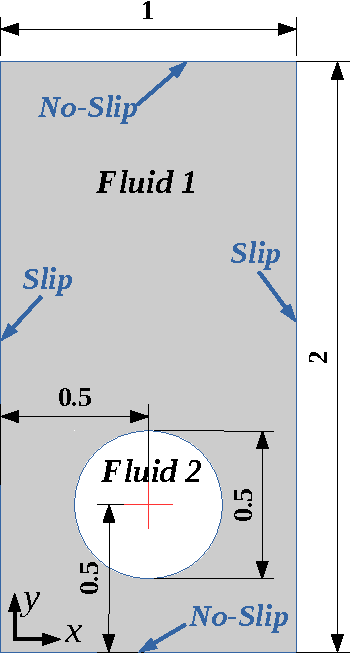
\includegraphics[width=4.25cm]{figures/benchmark_scheme.pdf}
 \vspace{-7mm}
\end{center}
\caption{Configuration and boundary conditions for 2D bubble benchmark.}
\label{benchmark_scheme}
\end{figure}
The 2D case setup is schematized in figure~\ref{benchmark_scheme}. First phase (liquid) properties are $\rho_1=1000$ kg/m$^3$, $\mu_1=10$ kg/(ms), while second phase (gas) takes $\rho_2=1$ kg/m$^3$, $\mu_2=0.1$ kg/(ms) as physical parameters. The surface tension is $\sigma=1.96$ kg/s$^2$. Gravity is taken as $g=0.98$ m/s$^2$. Extension of this test case to 3D is straightforward~\cite{Adelsberger2014}.

Uniform Cartesian 2D grids (cubic hexahedra) or triangular 2D grids (triangular prisms) cells were used for all simulations. The present work will only discuss 2D simulations. Six grid resolutions have been used ranging from 20 to 640 cells along the~$x$ direction, with the cell size halfed in each refinement. Hexahedral uniform grids were generated with the utility \verb+blockMesh+, while prismatic grids were created with Pointwise\textsuperscript{\textregistered} using mean edge size identical to the Cartesian grids. Grids are in the plane~$xy$ on a $1\times 2$ domain. The number of cells in the~$y$ direction is the double of that in the~$x$ direction. The bubble rises along the positive~$y$ direction. As OpenFOAM computations are always tridimensional, there is one single cell in the~$z$ direction, which has been taken of the same size as along~$x$ or~$y$.

The bubble was initialized as a cylinder in 2D using the \verb+setAlphaField+ utility. The Crank-Nicolson second order time scheme with blending coefficient 0.9 has been used for all computations. The convective term was treated with \verb+Gauss limitedlinearV 1+, and, in the MULES simulations, \verb+Gauss vanLeer+ was used for the $\alpha$ convection. The \verb+Gauss linear+ scheme was used for gradient terms on hexahedral grids while \verb+pointCellsLeastSquares+ was used for prismatic meshes. The GAMG implicit solver was used for pressure terms, while the smooth solver was used for the velocity. Constant time steps have been used, starting at $\Delta t=0.002$ s for the coarsest level and reduced for finer grids to keep the maximum CFL number below 0.05. The PIMPLE algorithm was run with \verb+nOuterCorrectors+ set to 3 and with 3 PISO correctors (\verb+nCorrectors+ set to 3). Setting \verb+momentumPredictor+ to \verb+true+ was necessary for accuracy with isoAdvector. The number of non-orthogonal correctors (\verb+nNonOrthogonalCorrectors+) was set to 1 on prismatic grids, 0 on hexahedral grids. Computations were run up to physical time $t=3$~s in 2D. 

\subsection{Results and discussion}\label{sec_hysingresults}
%%-----------------------------------------------------------------
Post-processing quantities of interest are described in details in~\cite{Hysing2009,Adelsberger2014}. These are the vertical position of the bubble centroid, the bubble rise velocity, the bubble circularity, area and volume. The volume of the bubble~$V_b$ is computed by a integral of the gas volume fraction over the entire domain~$\Omega$ as: 
\begin{equation}
  V_b = \int_{\Omega} (1-\alpha)\,dv
\end{equation}

The centroid of mass~$\overrightarrow{x_G}$ is computed through: 
\begin{equation}
  \overrightarrow{x_G} = \frac{1}{V_b}~\int_{\Omega}(1-\alpha)\overrightarrow{x}\,dv
\end{equation}
where $\overrightarrow{x}$ represents the cell center coordinates. Similarly, the bubble velocity is calculated with:
\begin{equation}
  \overrightarrow{U_b} = \frac{1}{V_b}~\int_{\Omega}(1-\alpha)\overrightarrow{U}\,dv
  \label{eqnPPvelocity}
\end{equation}
where $\overrightarrow{U}$ denotes the mixture velocity, which is stored at cell centers in OpenFOAM. The bubble area~$A_b$ is determined by using the method \verb+area+ of the C++ class \verb+sampledIsoSurfaceCell+ to compute the isosurface $\alpha=0.5$. The circularity~$\cal{C}$ is then defined as the ratio of the equivalent radius of the bubble based on its volume~$r_V$, over the equivalent radius of the bubble based on its surface~$r_A$. Since we are in 2D, we obtain: 
\begin{equation}
 {\cal{C}} = \frac{r_V}{r_A} = \frac{\sqrt{V_b/(\pi \Delta_z)}}{ A_b/(2 \pi \Delta_z)} 
\end{equation}
where $\Delta_z$ denotes the size of the grid cells in the non-significant direction~$z$. The circularity~$\cal{C}$ takes the value 1 at the beginning of the computation and decreases as the bubble deforms.

\begin{figure}[!h]
\begin{center}
 \vspace{-1mm}
 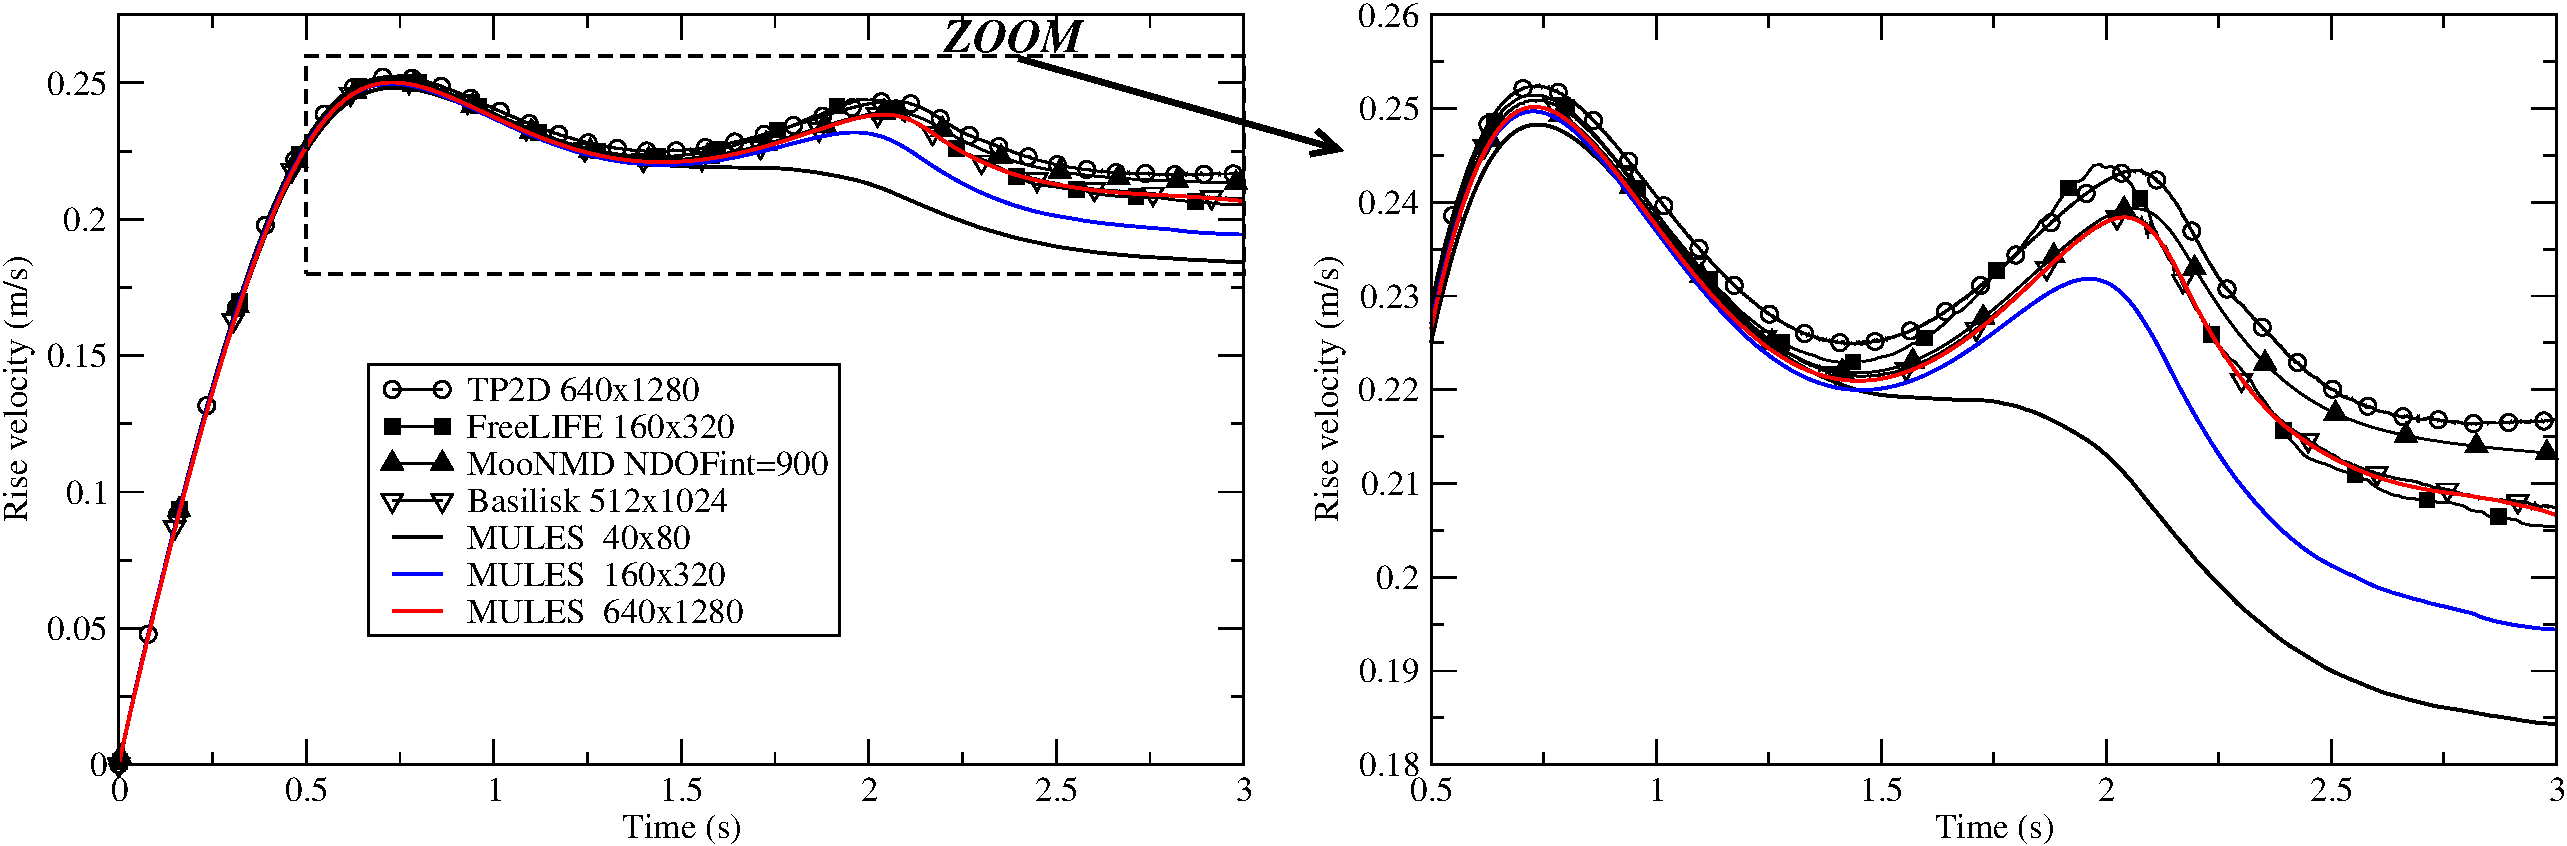
\includegraphics[width=\textwidth]{figures/HysingB_bubble_velocity_MULES.pdf}
 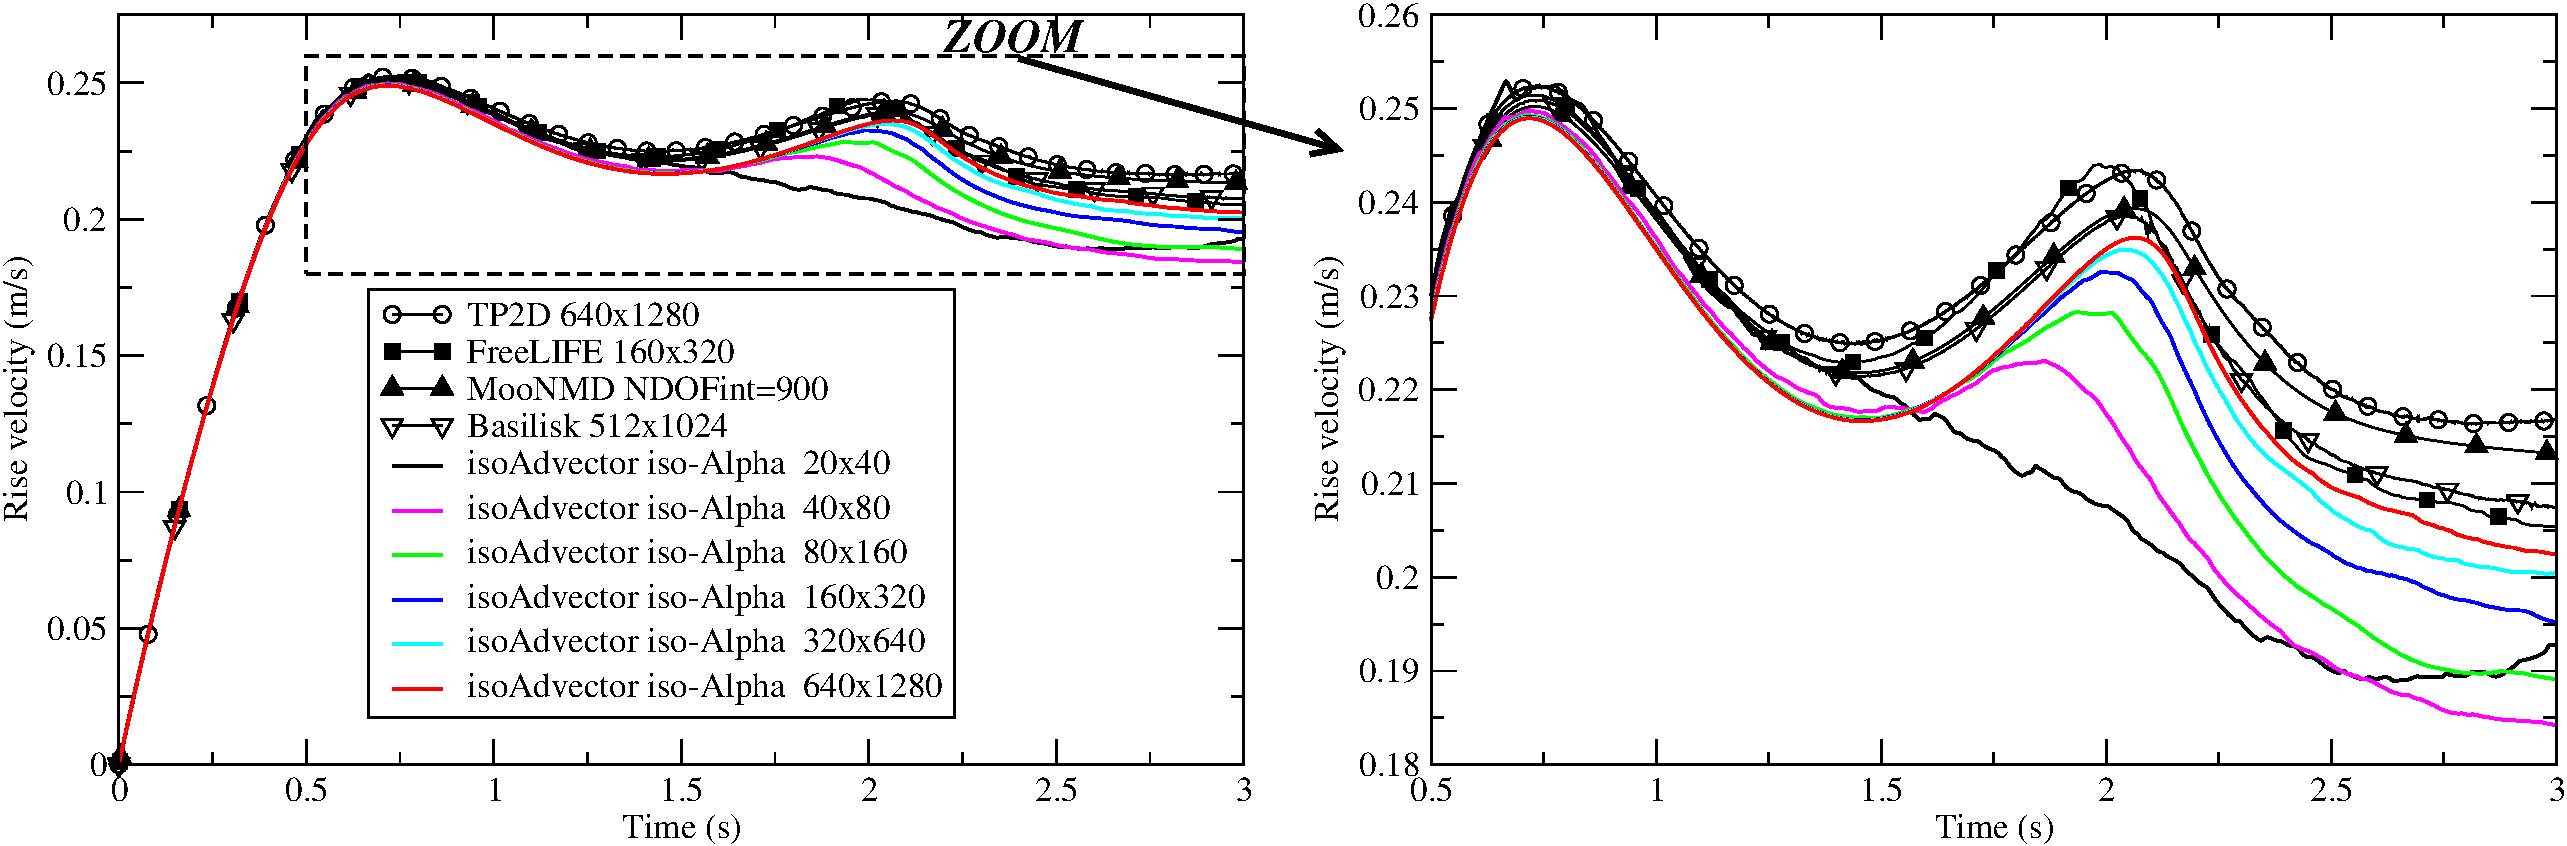
\includegraphics[width=\textwidth]{figures/HysingB_bubble_velocity_isoAlpha.pdf}
 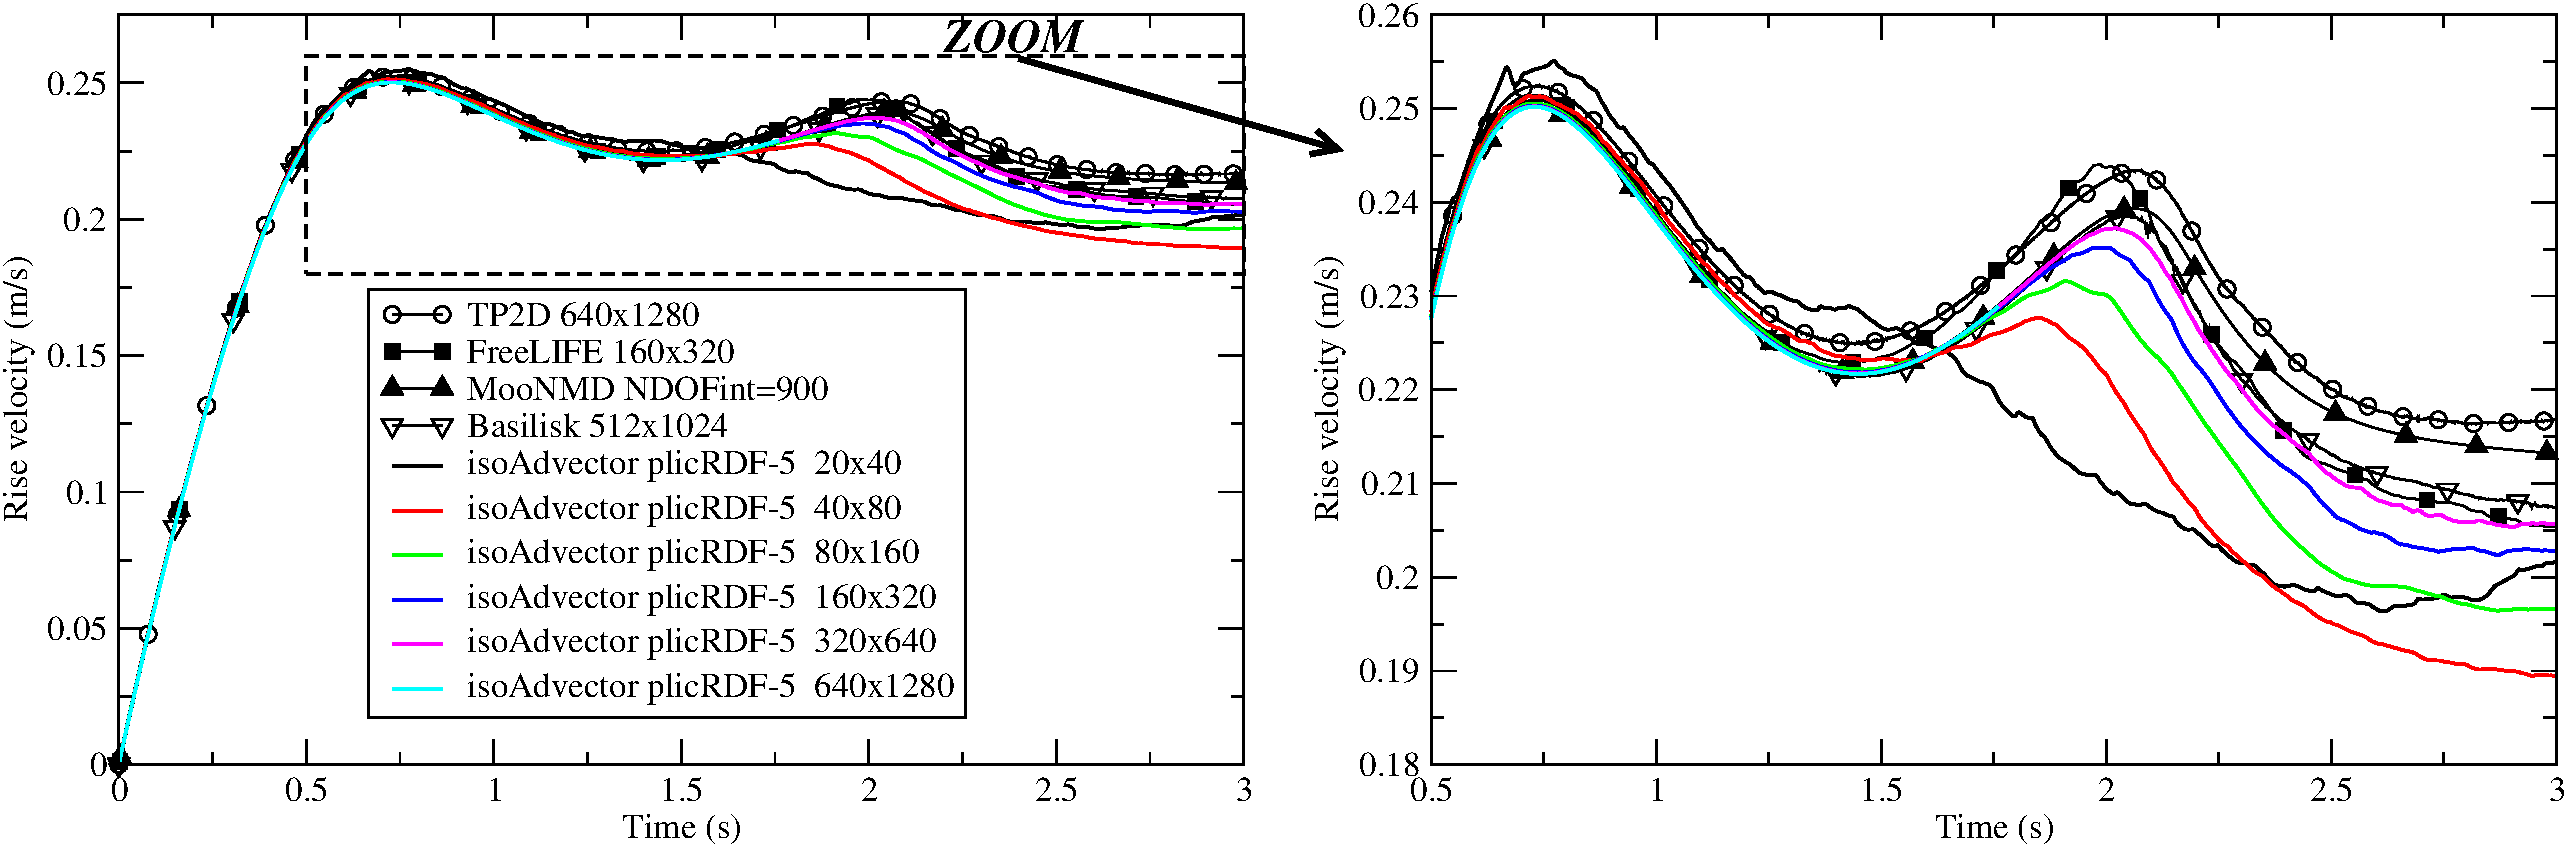
\includegraphics[width=\textwidth]{figures/HysingB_bubble_velocity_plicRDF5.pdf}
 \vspace{-14mm}
\end{center}
\caption{Time evolution of rise velocity on hexahedral grids for solvers MULES (top), isoAdvector with isoAlpha (middle) and plicRDF-5 (botttom) reconstruction schemes.}
\label{fig:HB_Struct_bubble_velocity}
\end{figure}

\begin{figure}[!h]
\begin{center}
 \vspace{-1mm}
 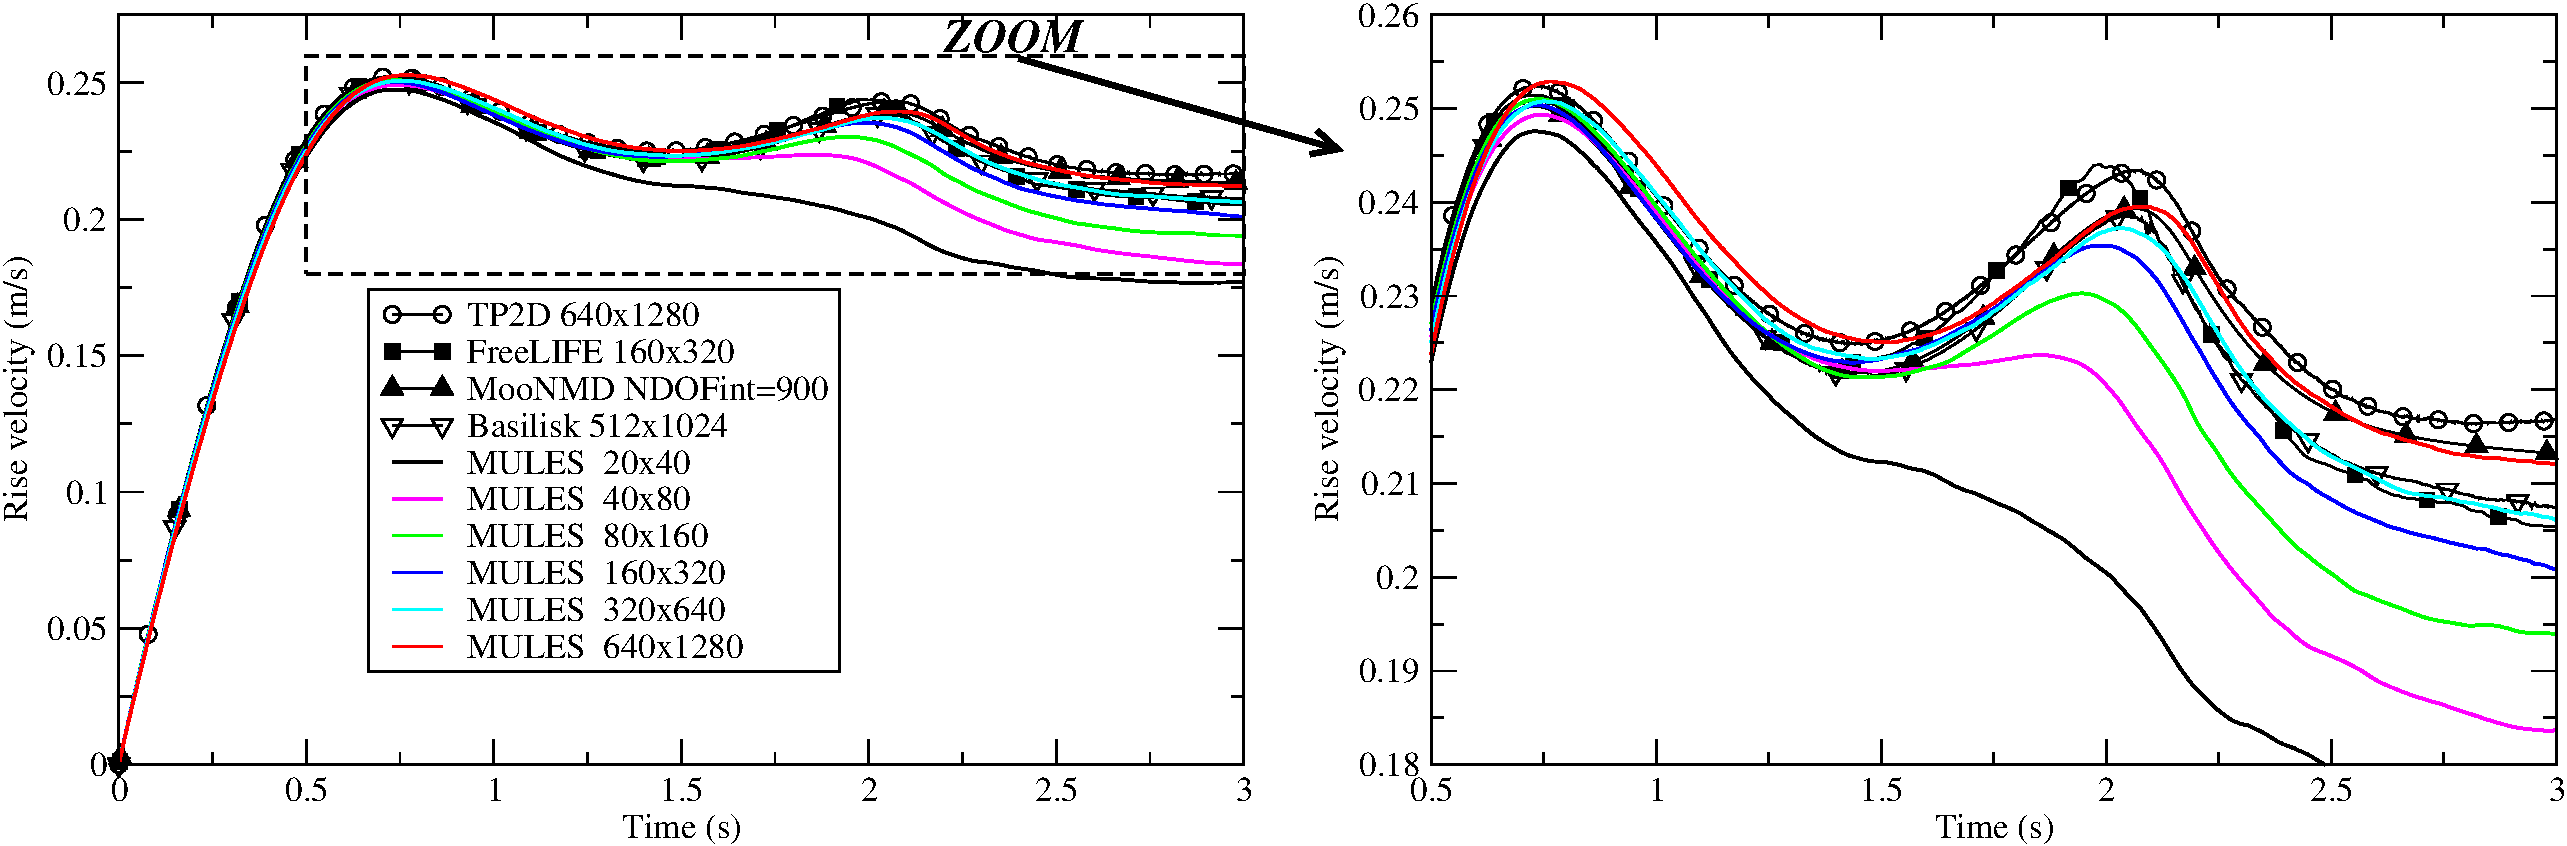
\includegraphics[width=\textwidth]{figures/HysingB-uns_bubble_velocity_MULES.pdf}
 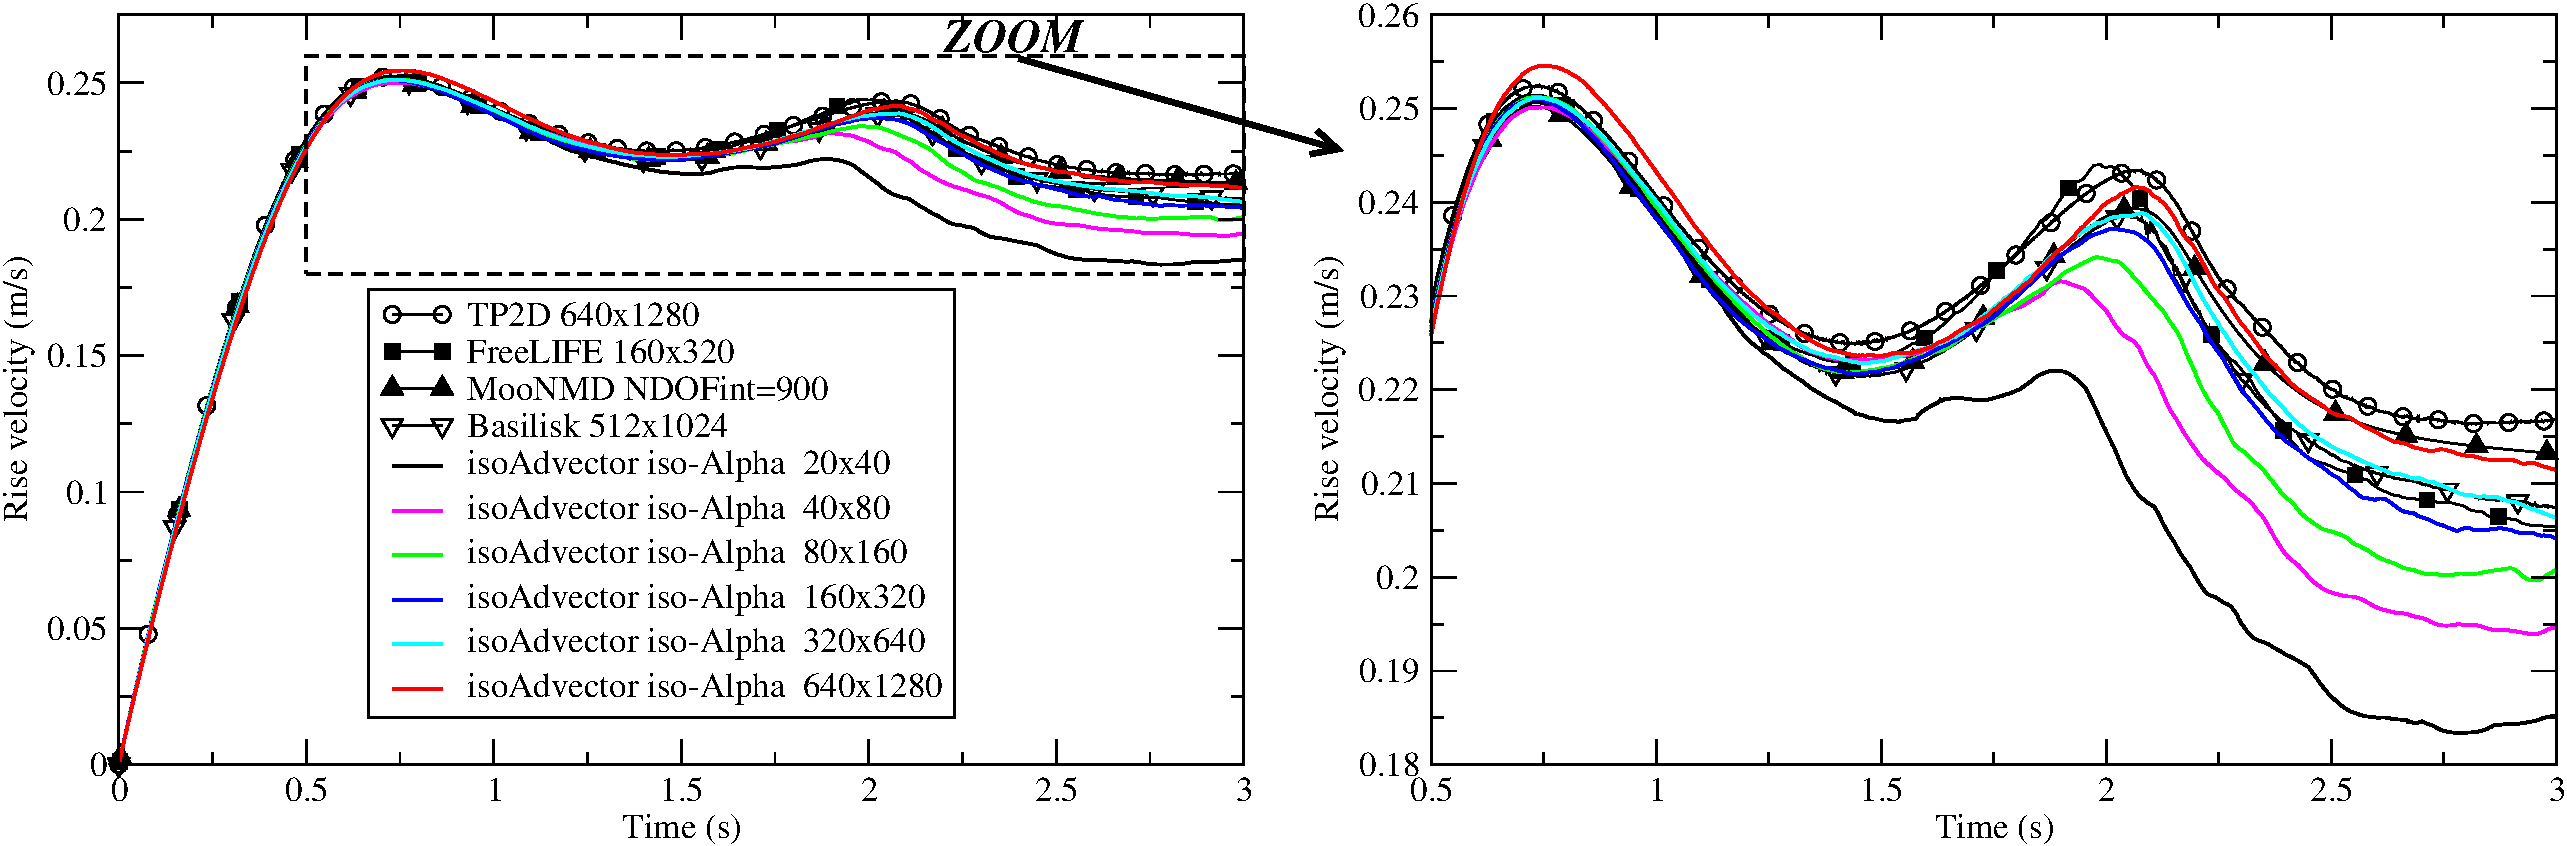
\includegraphics[width=\textwidth]{figures/HysingB-uns_bubble_velocity_isoAlpha.pdf}
 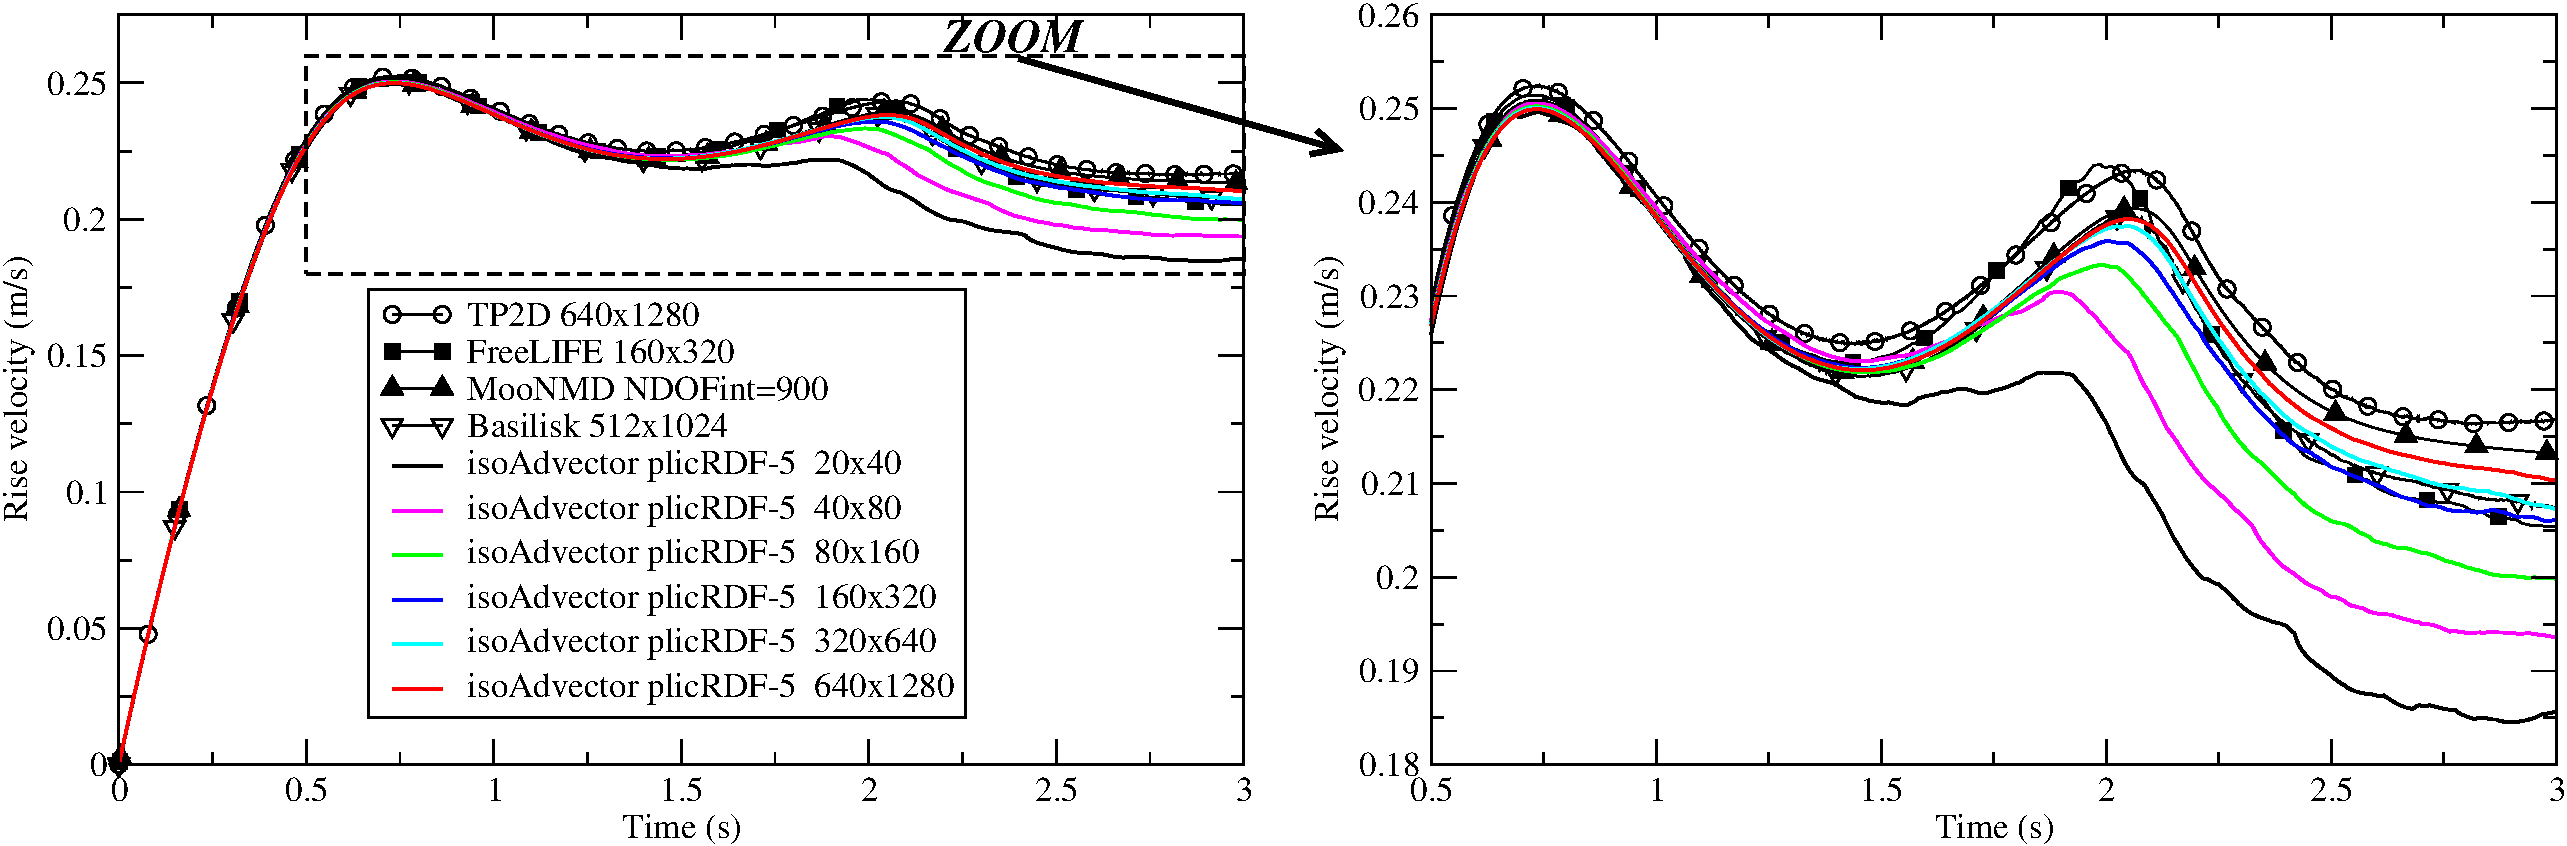
\includegraphics[width=\textwidth]{figures/HysingB-uns_bubble_velocity_plicRDF5.pdf}
 \vspace{-14mm}
\end{center}
\caption{Time evolution of rise velocity on triangular grids for solvers MULES (top), isoAdvector with isoAlpha (middle) and plicRDF5 (botttom) reconstruction schemes.}
\label{fig:HB_Uns_bubble_velocity}
\end{figure}
 
The figure~\ref{fig:HB_Struct_bubble_velocity} shows results for the rise velocity for MULES, isoAdvector isoAlpha and plicRDF-5 on hexahedral grids compared to the highest resolution reference data available in the literature. We first note that grid convergence is reached by all three OpenFOAM solvers. MULES and plicRDF-5 results are rather similar, while isoAlpha results converge to a slightly different solution. The figure~\ref{fig:HB_Uns_bubble_velocity} shows results on triangular grids. At higher grid resolutions, we clearly notice that neither MULES nor isoAlpha reach a grid convergence, showing overestimated bubble velocities (see red curve). This behavior can be explained by an increase of spurious currents at highest grid resolutions for these methods. The integral procedure to compute bubble velocity of equation~\ref{eqnPPvelocity} inherently accounts for spurious currents in the solution. Spurious currents will be discussed in more details hereafter in section~\ref{sec_spuriouscase} in the objective to quantify their effect on the solution. 

Figure~\ref{fig:HB_bubble_shape_3_others} shows the bubble shape at time $t=3$ obtained by reference solvers of the literature. It can first be noted that every code gives a different solution, particularly in the trains of detached bubbles. As a matter of fact, the test case number 2 of the benchmark of Hysing~\cite{Hysing2009} is more challenging to simulate than test case 1. Figures~\ref{fig:HB_bubble_shape_3_MULES}, \ref{fig:HB_bubble_shape_3_isoAlpha} and~\ref{fig:HB_bubble_shape_3_plicRDF5} compare the bubble shapes for respectively MULES, isoAlpha and plicRDF-5, for two grid resolutions, either on hexahedral or prismatic meshes. All bubble shapes for all solvers are rather coherent in terms of global positions of the main leading and trailing fronts. For each solver of figures~\ref{fig:HB_bubble_shape_3_MULES}, \ref{fig:HB_bubble_shape_3_isoAlpha} and~\ref{fig:HB_bubble_shape_3_plicRDF5}, the trains of detached bubbles are different between hexahedral and prismatic grids. The OpenFOAM finest grids results are close to MooNMD and Basilik shapes, as plotted on figure~\ref{fig:HB_bubble_shape_3_others}. 

Circularity is shown on figures~\ref{fig:HB_bubble_circularity160} and~\ref{fig:HB_bubble_circularity640}, at respective grid resolutions 160x320 and 640x1280. OpenFOAM solvers compare well to reference data, except with the TP2D solver which experiences a different bubble tail structure (see also top left plot in figure~\ref{fig:HB_bubble_shape_3_others}). The difference between square (continuous lines) and triangular (dashed lines) grids on MULES, isoAlpha or plicRDF-5 circularities is more visible for time $t>2$ up to the end of the simulation. This is mainly due to the difference in the bubble tail, discussed hereafter. 

For completeness about the bubble shape at time $t=3$, we show on figures~\ref{fig:HB_compareOFMULES_Fineststruct.vs.uns}, \ref{fig:HB_compareOFisoAlpha_Fineststruct.vs.uns} and~\ref{fig:HB_compareOFplicRDF5_Fineststruct.vs.uns} a comparison of the bubble shape on increasing size triangular grids with respect to the finest Cartesian grid shape made with the same solver. MULES and plicRDF-5 show a correct grid convergence. At the finest levels (320x640 and 640x1280), square and triangular grids are almost identical, particularly in their main fronts. One should however notice a small discrepancy in the upper front for the MULES solver at 640x1280 (see figure~\ref{fig:HB_compareOFMULES_Fineststruct.vs.uns}). For the isoAlpha solver, the difference between square and triangular grids remains for all levels, and even increases slightly at the highest resolution.

Figure~\ref{fig:HB_bubble_shape_time_evol_uns080_MULES_vs_plicRDF5} (resp.~\ref{fig:HB_bubble_shape_time_evol_uns320_MULES_vs_plicRDF5}) shows a typical time sequence of bubble shape, plotted every 0.5s, on a 80x160 (resp. 320x640) hexahedral grid, for solvers MULES and plicRDF-5. Differences between the two solvers are only visible after time $t=2.5$. Besides, increasing the resolution blurs these differences. 

\begin{figure}[!h]
\begin{center}
 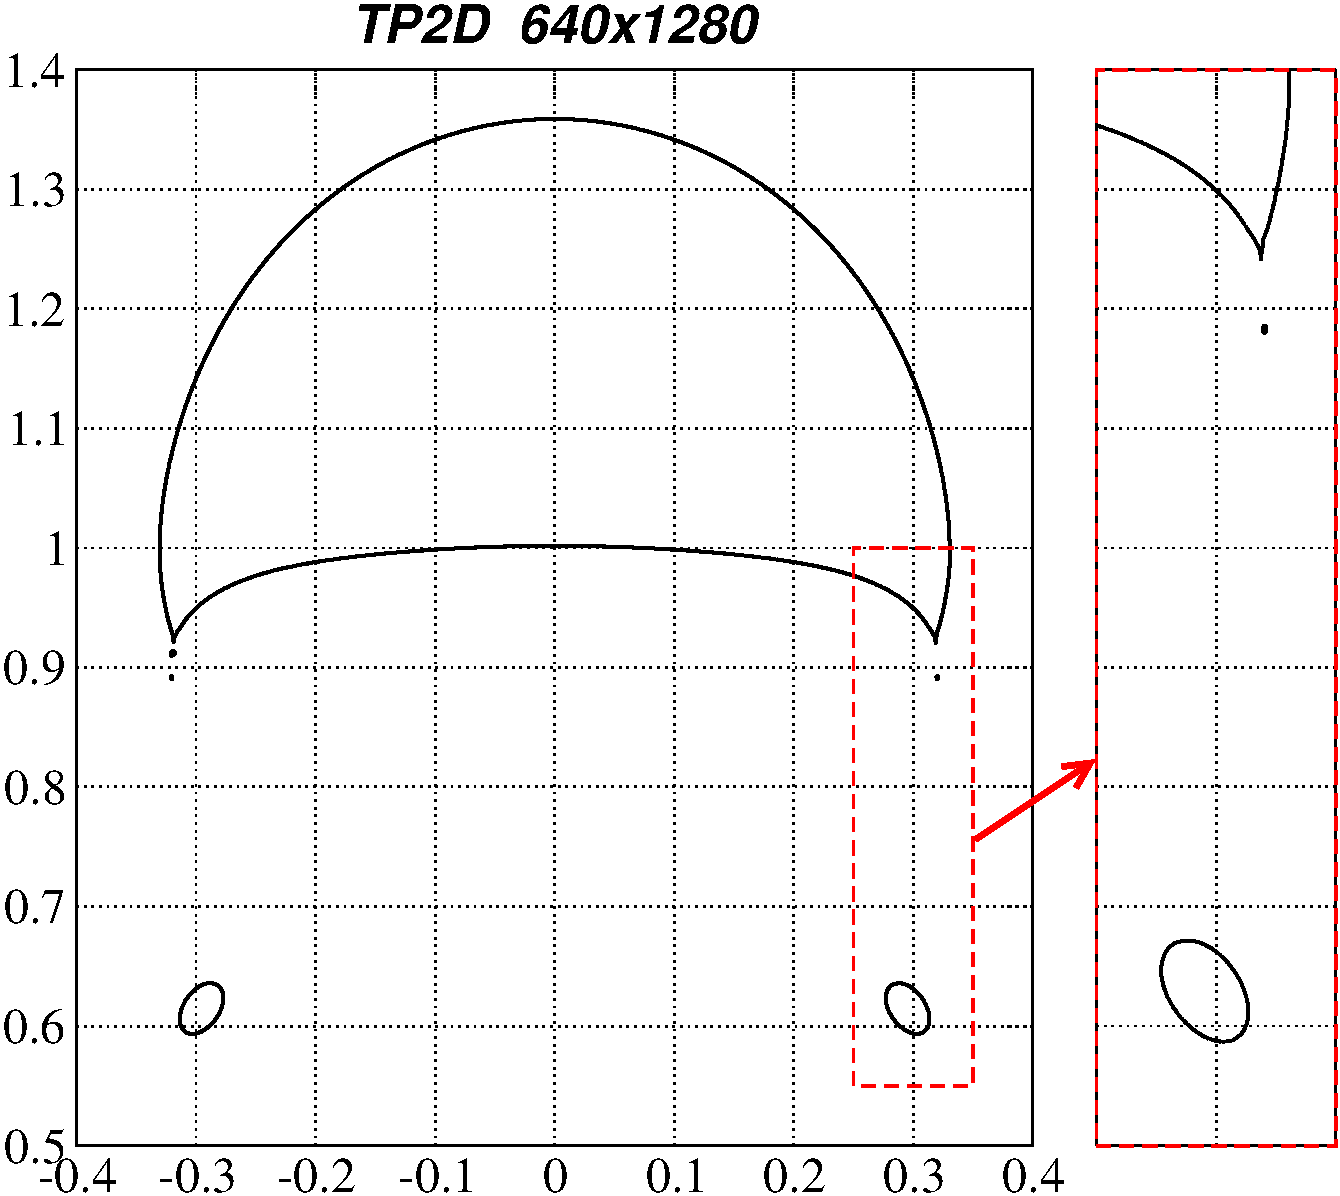
\includegraphics[width=0.45\textwidth]{figures/bubble_shape_t=3_TP2D.pdf}
 \hspace{4mm}
 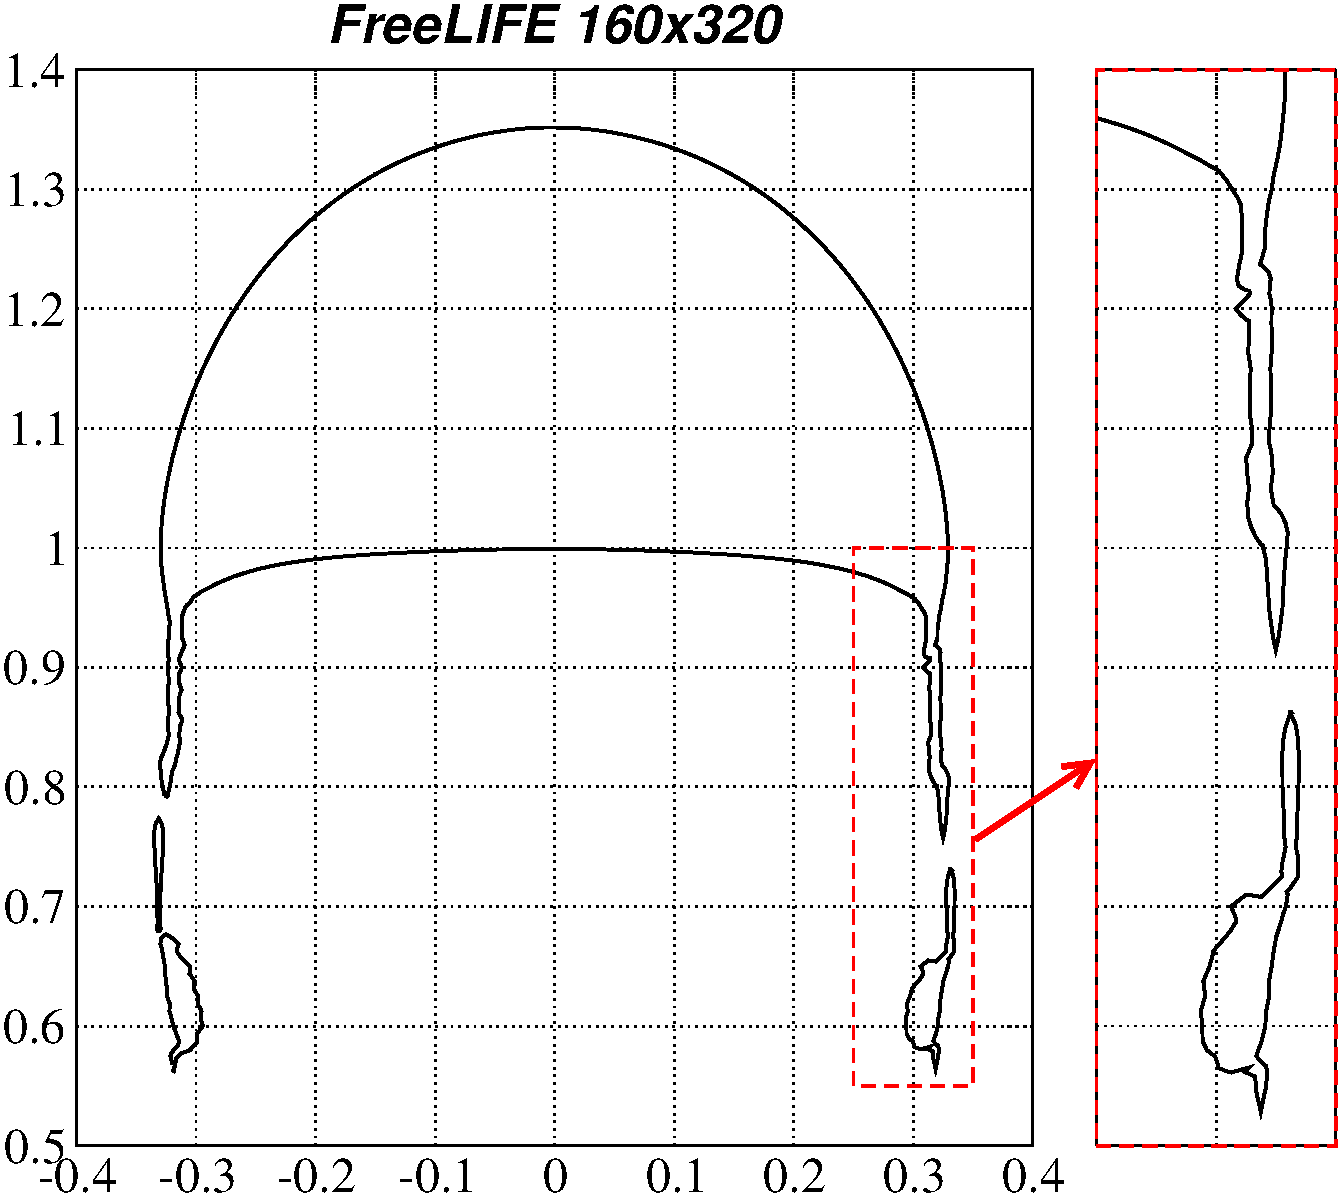
\includegraphics[width=0.45\textwidth]{figures/bubble_shape_t=3_FreeLIFE.pdf}

 \vspace{2mm}

 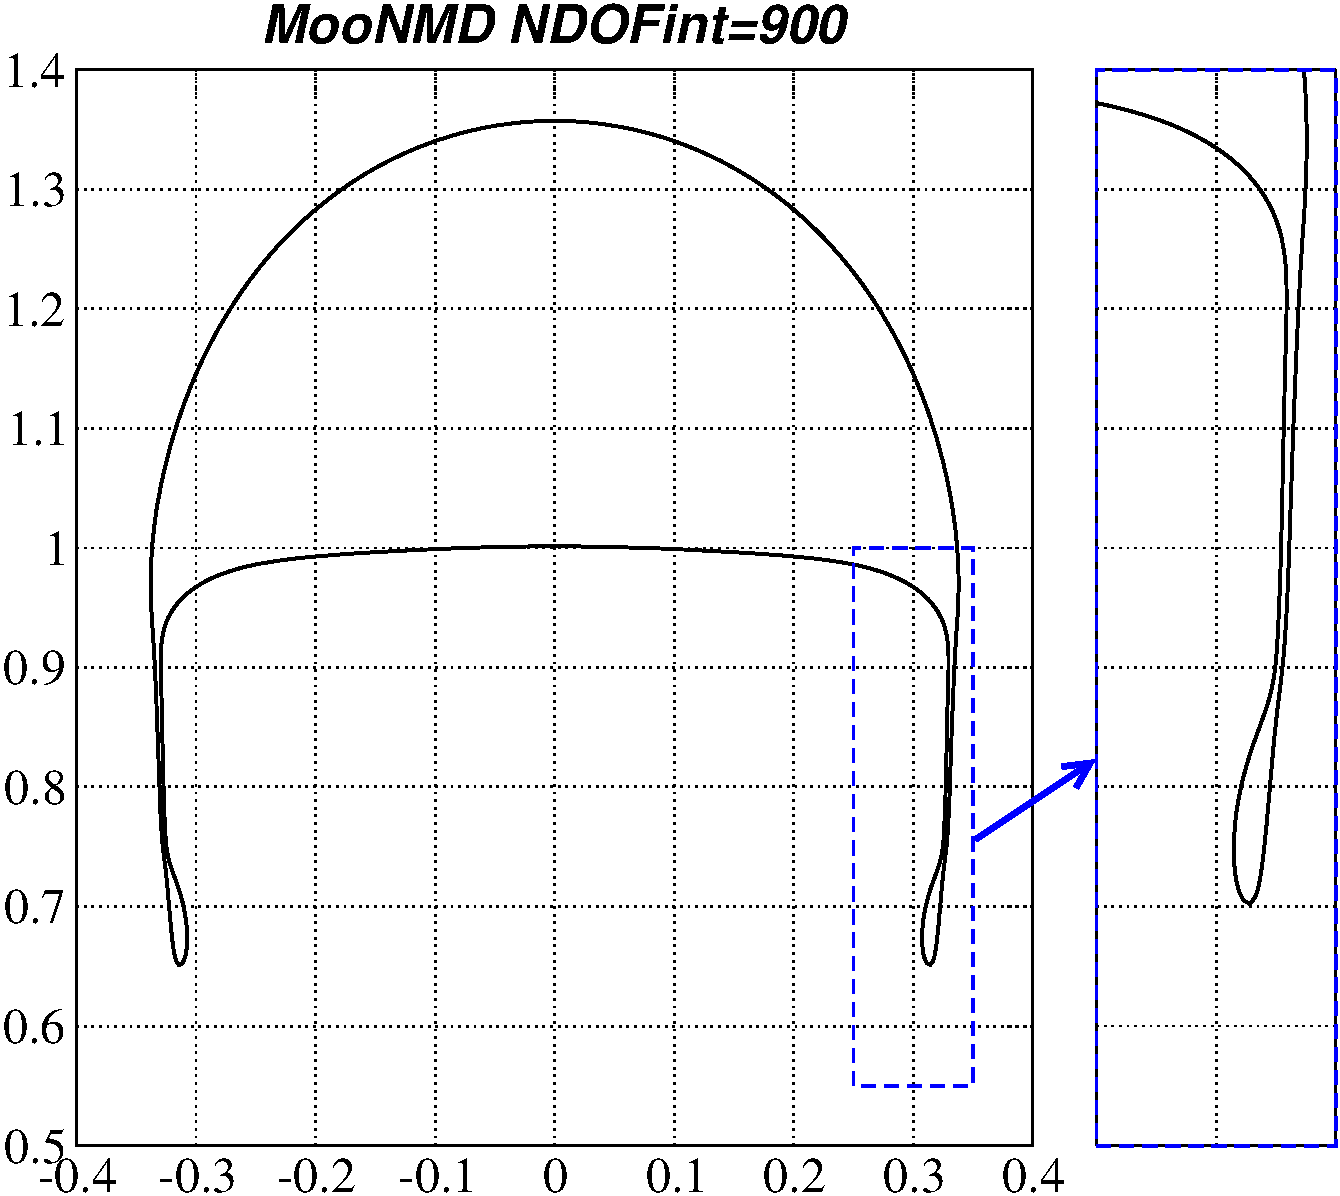
\includegraphics[width=0.45\textwidth]{figures/bubble_shape_t=3_MoonNMD.pdf}
 \hspace{4mm}
 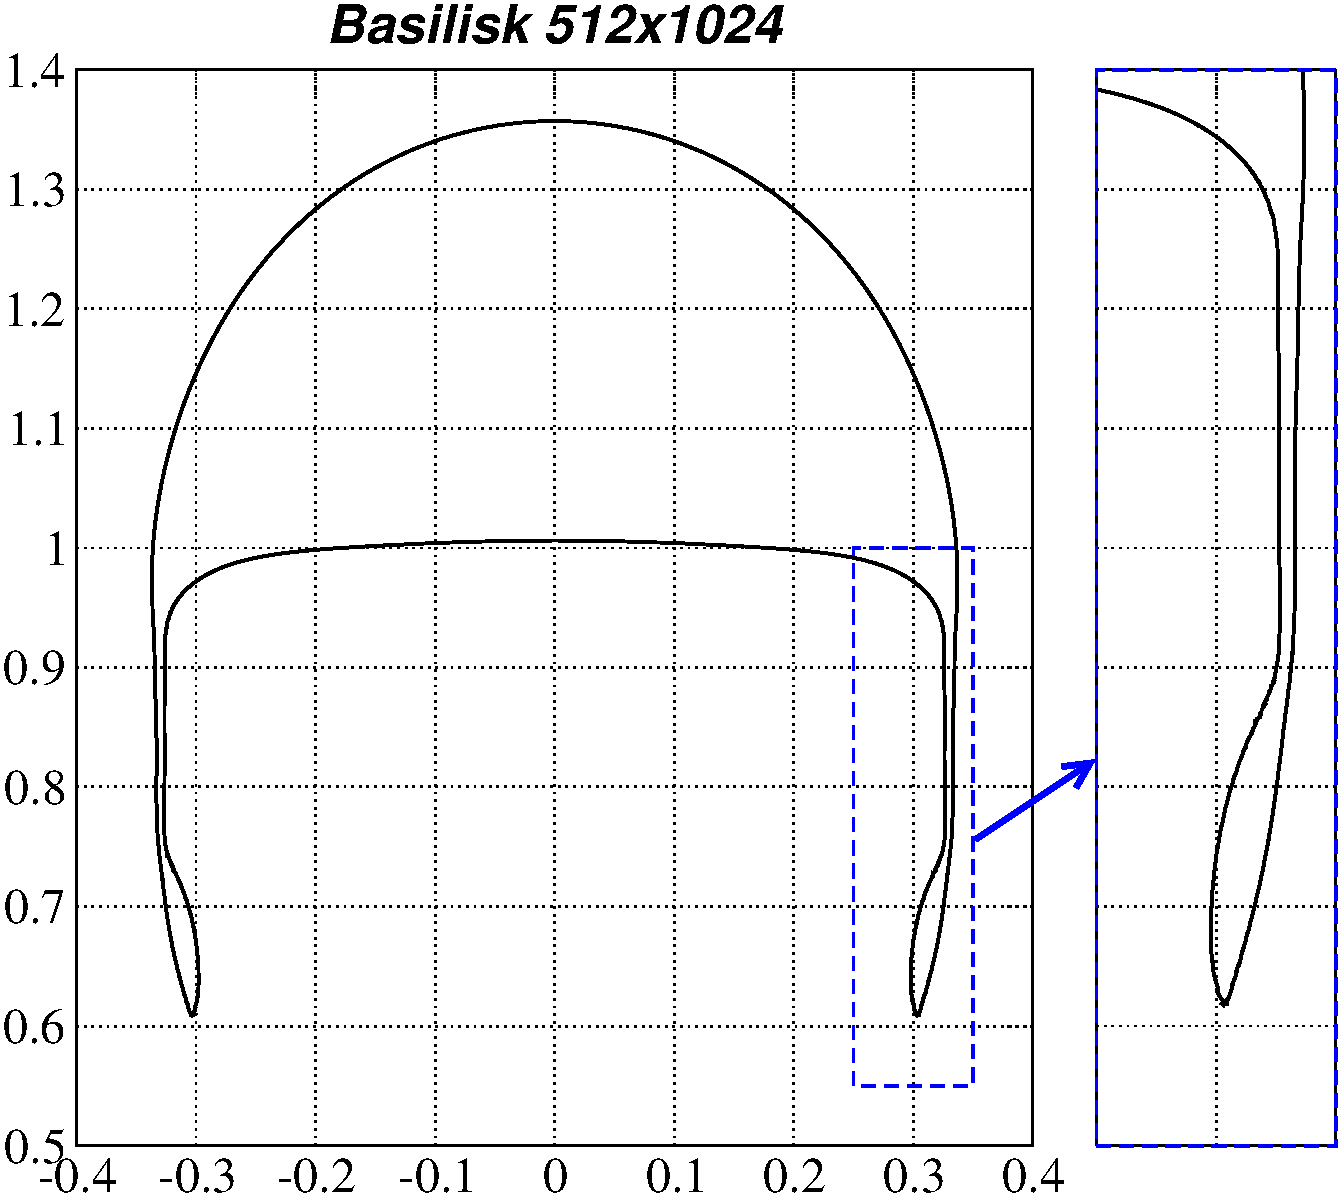
\includegraphics[width=0.45\textwidth]{figures/bubble_shape_t=3_Basilisk.pdf}
 
 \vspace{-6mm}
\end{center}
\caption{Bubble shape at time t=3 for TP2D, FreeLIFE, MoonNMD and Basilisk solvers.}
\label{fig:HB_bubble_shape_3_others}
\end{figure}


\begin{figure}[!h]
\begin{center}
 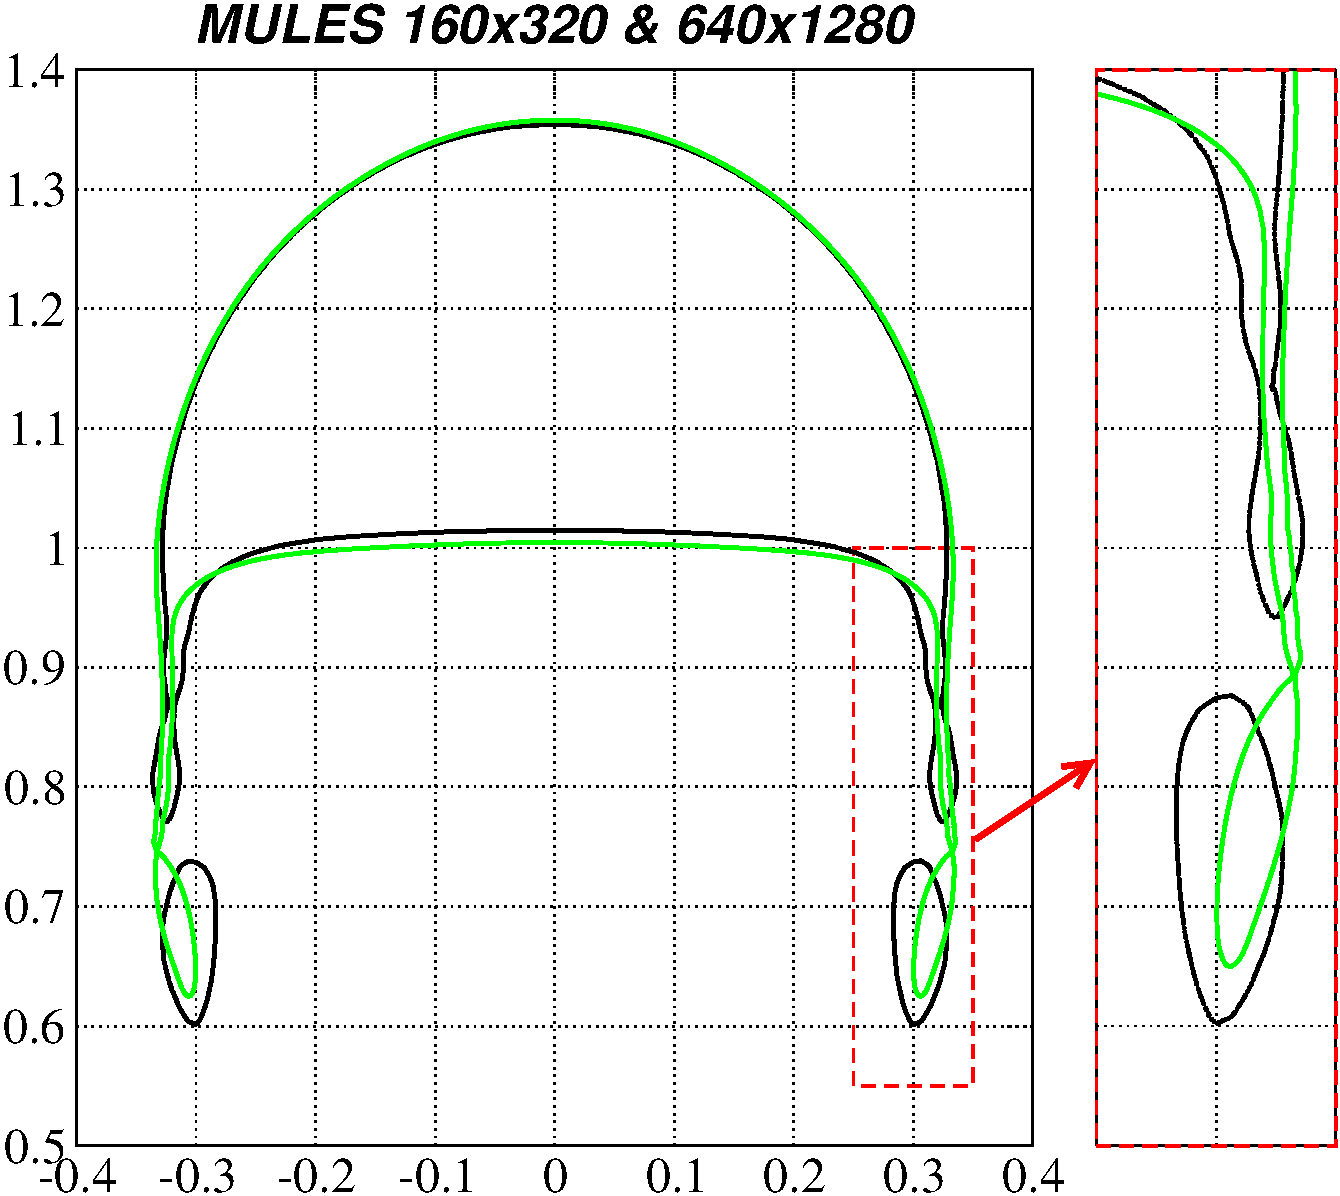
\includegraphics[width=0.45\textwidth]{figures/bubble_shape_t=3_MULES-struct.pdf}
 \hspace{2mm}
 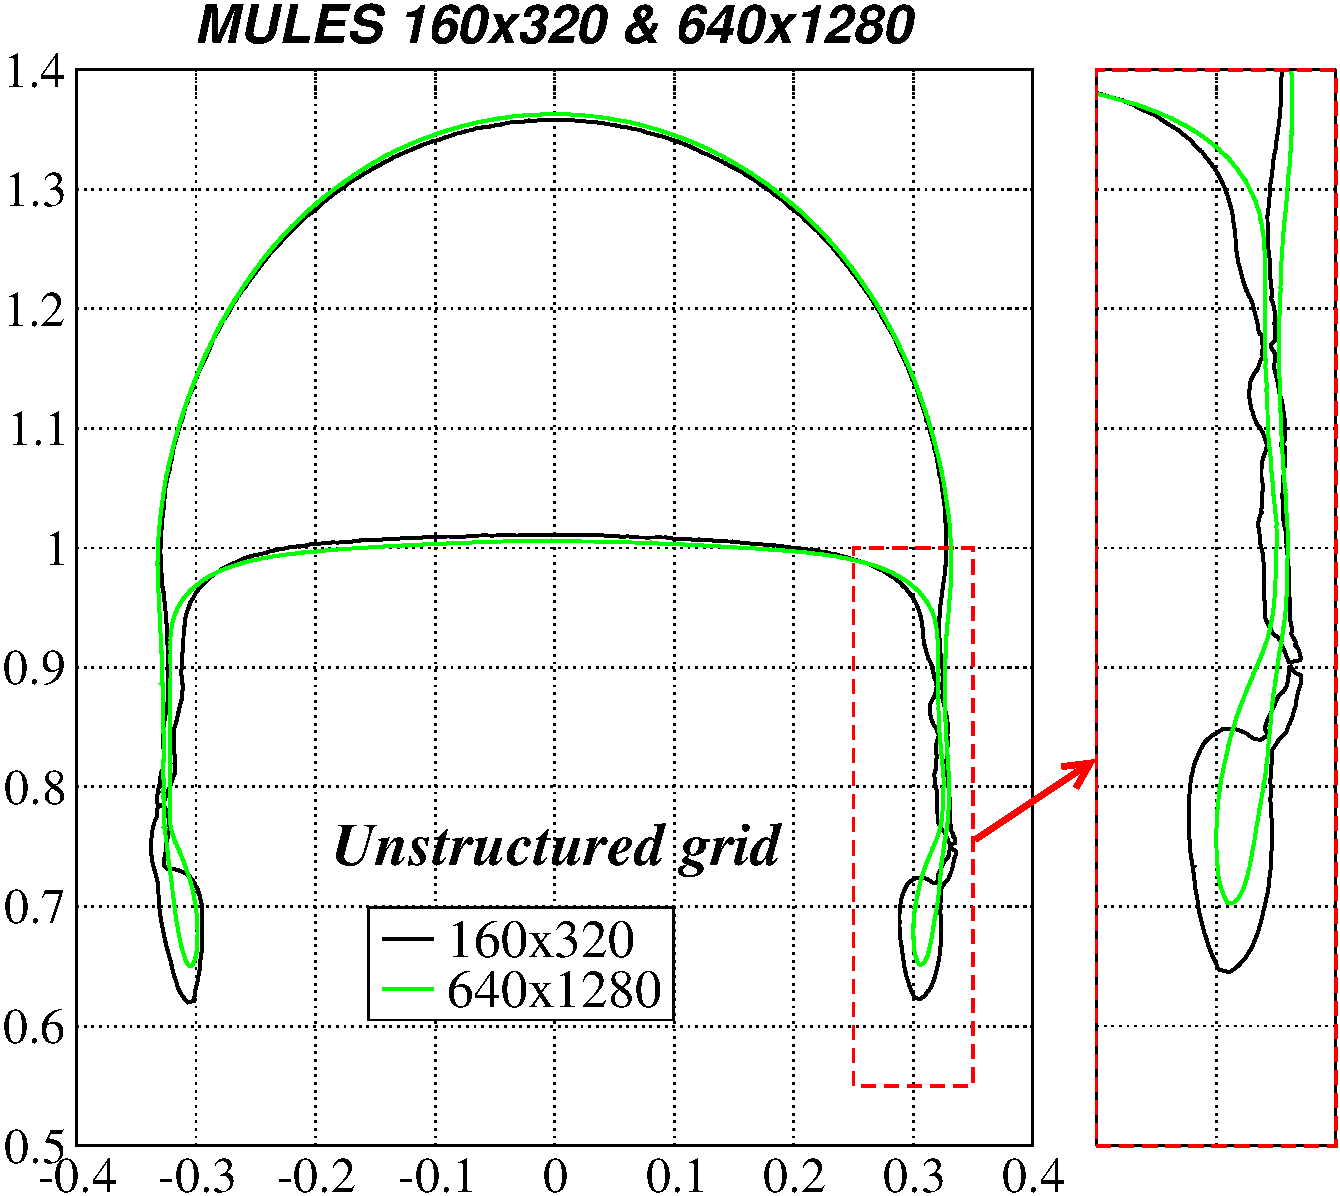
\includegraphics[width=0.45\textwidth]{figures/bubble_shape_t=3_MULES-uns.pdf}
 \vspace{-6mm}
\end{center}
\caption{Bubble shape at time t=3 for MULES. Left: square grids, Right: triangular.}
\label{fig:HB_bubble_shape_3_MULES}
\end{figure}

\begin{figure}[!h]
\begin{center}
 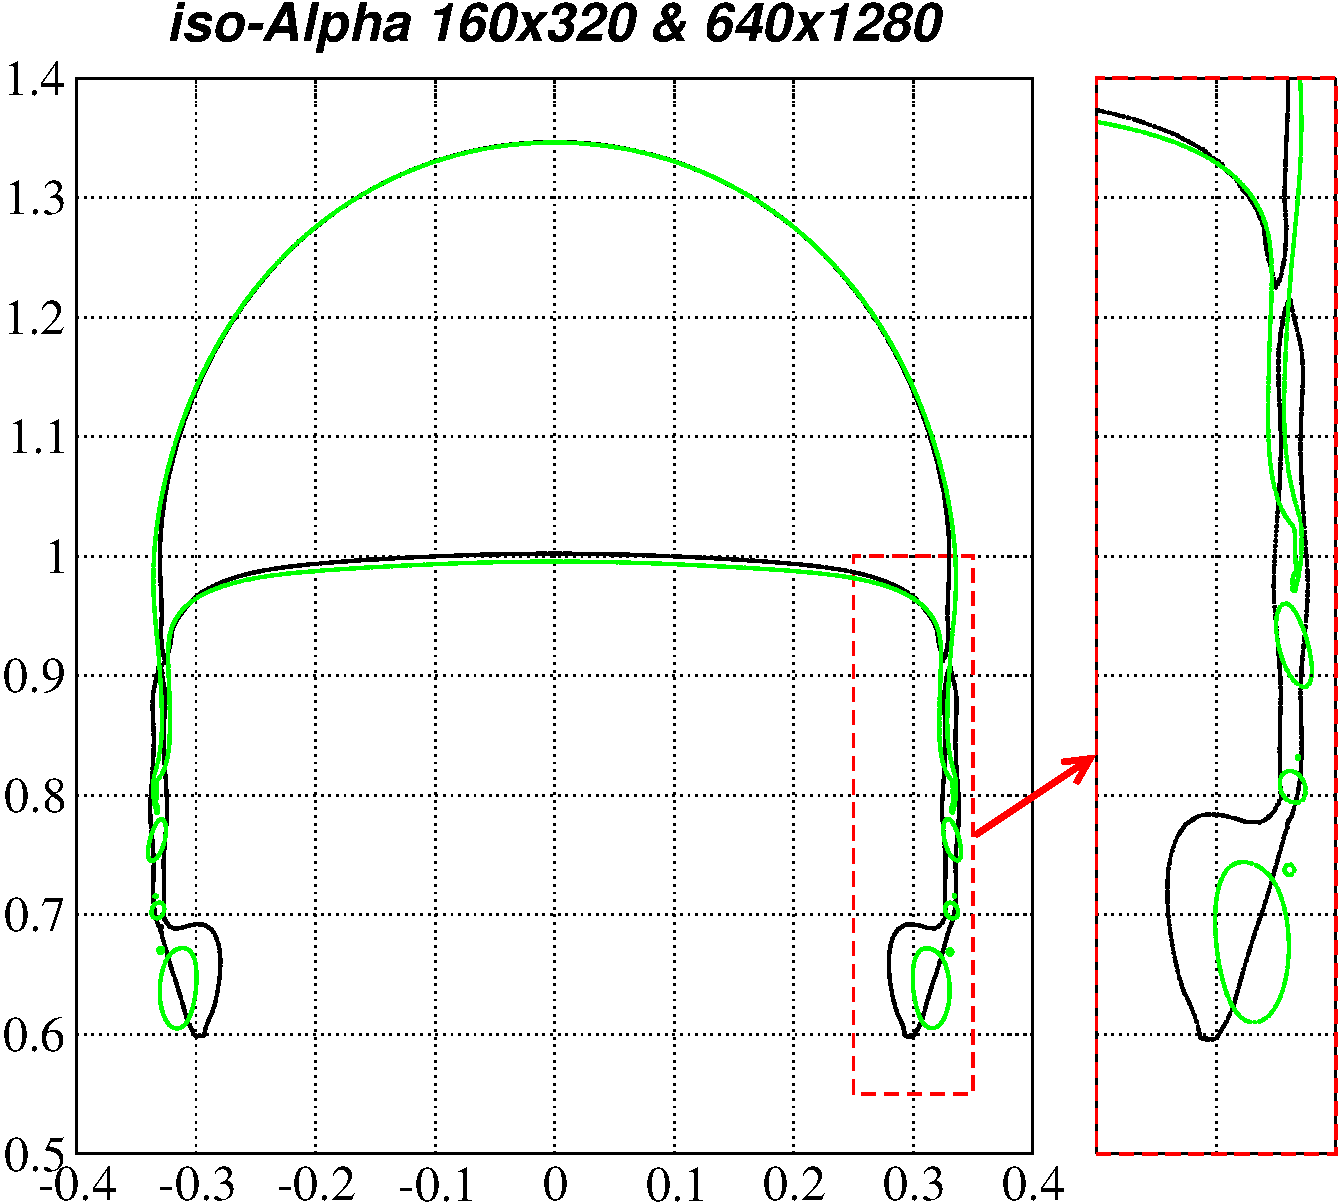
\includegraphics[width=0.45\textwidth]{figures/bubble_shape_t=3_isoAlpha-struct.pdf}
 \hspace{2mm}
 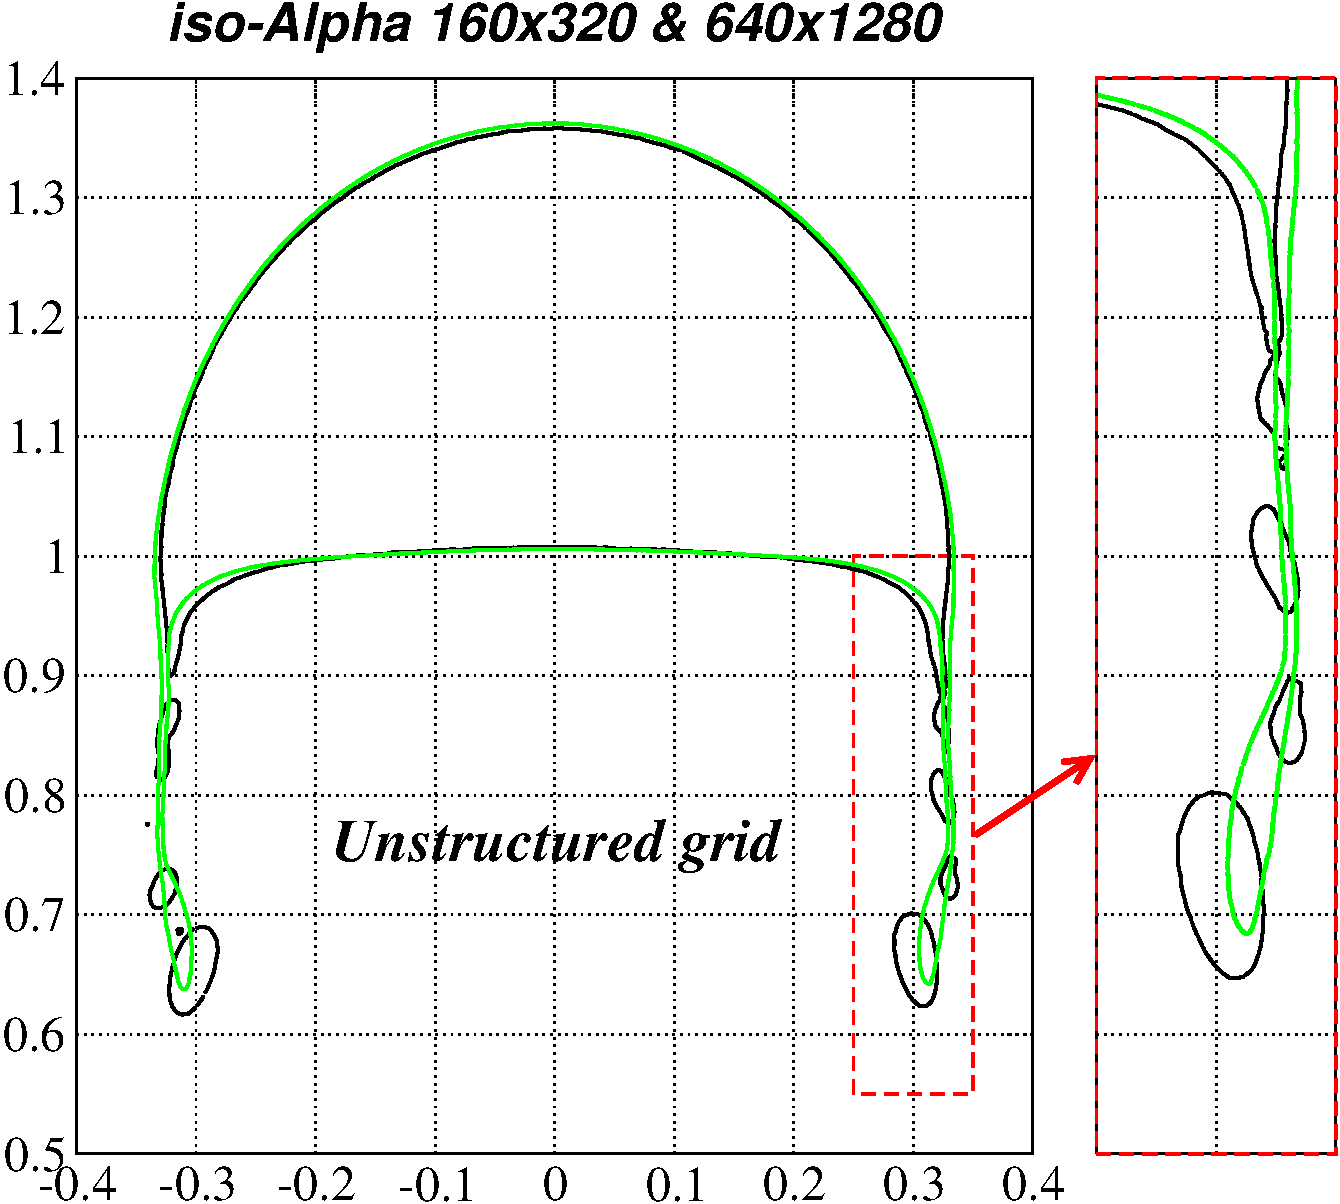
\includegraphics[width=0.45\textwidth]{figures/bubble_shape_t=3_isoAlpha-uns.pdf}
 \vspace{-6mm}
\end{center}
\caption{Bubble shape at time t=3 for isoAdvector isoAlpha. Left: square grids, Right: triangular.}
\label{fig:HB_bubble_shape_3_isoAlpha}
\end{figure}

\begin{figure}[!h]
\begin{center}
 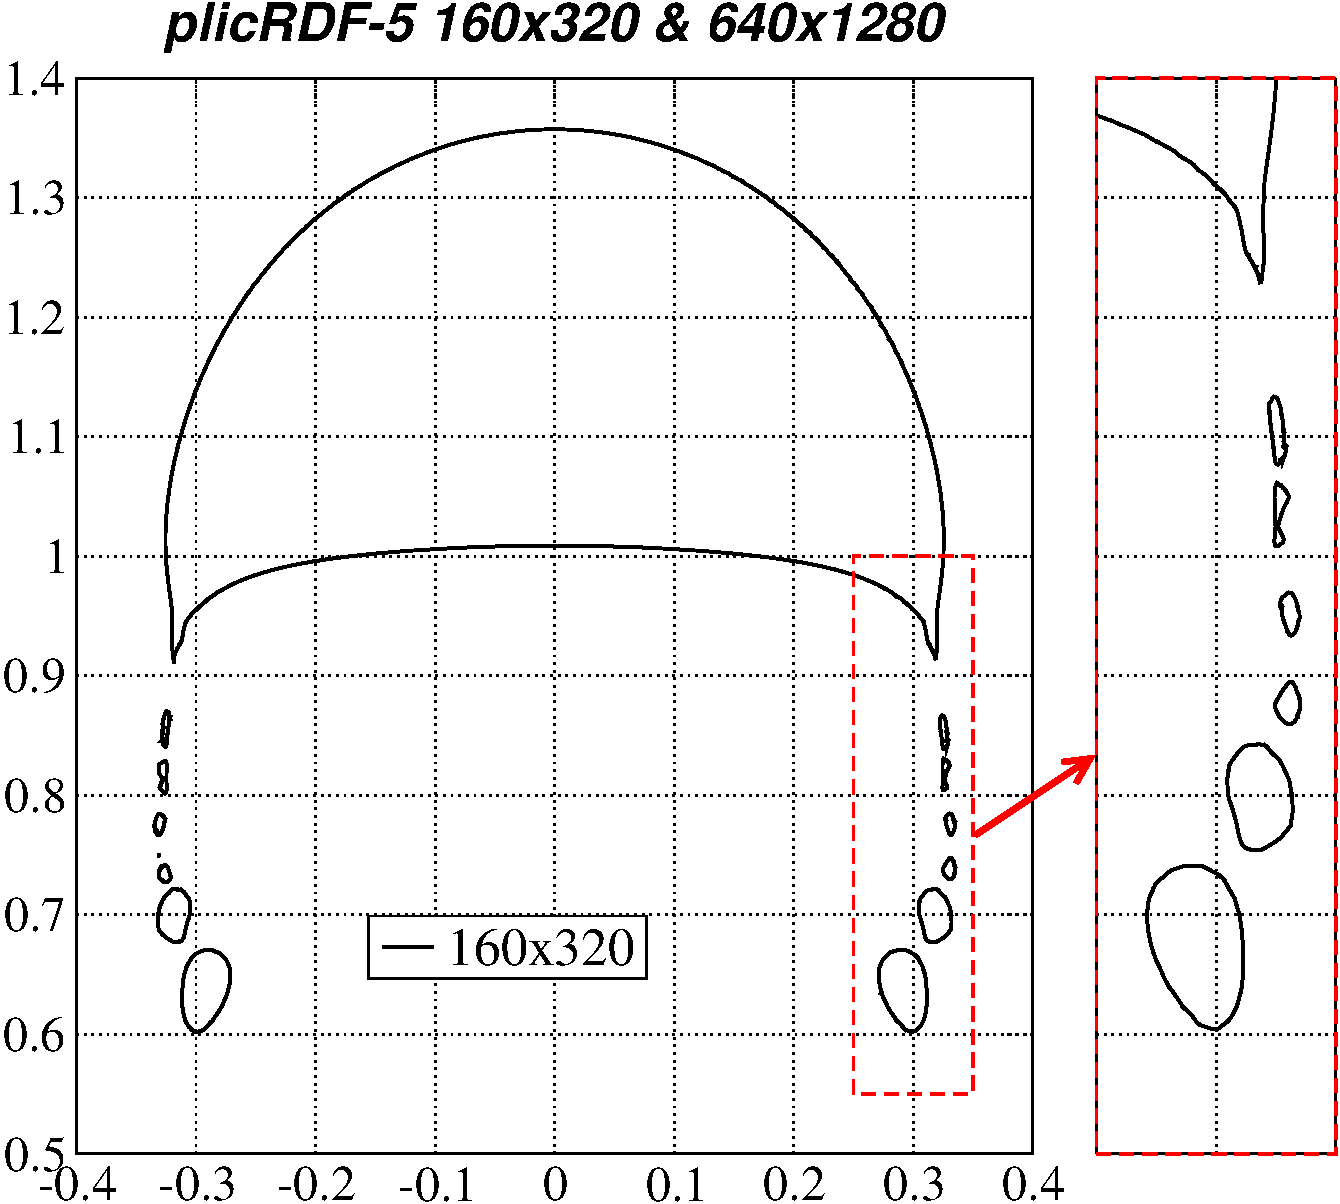
\includegraphics[width=0.45\textwidth]{figures/bubble_shape_t=3_plicRDF5-struct.pdf}
 \hspace{2mm}
 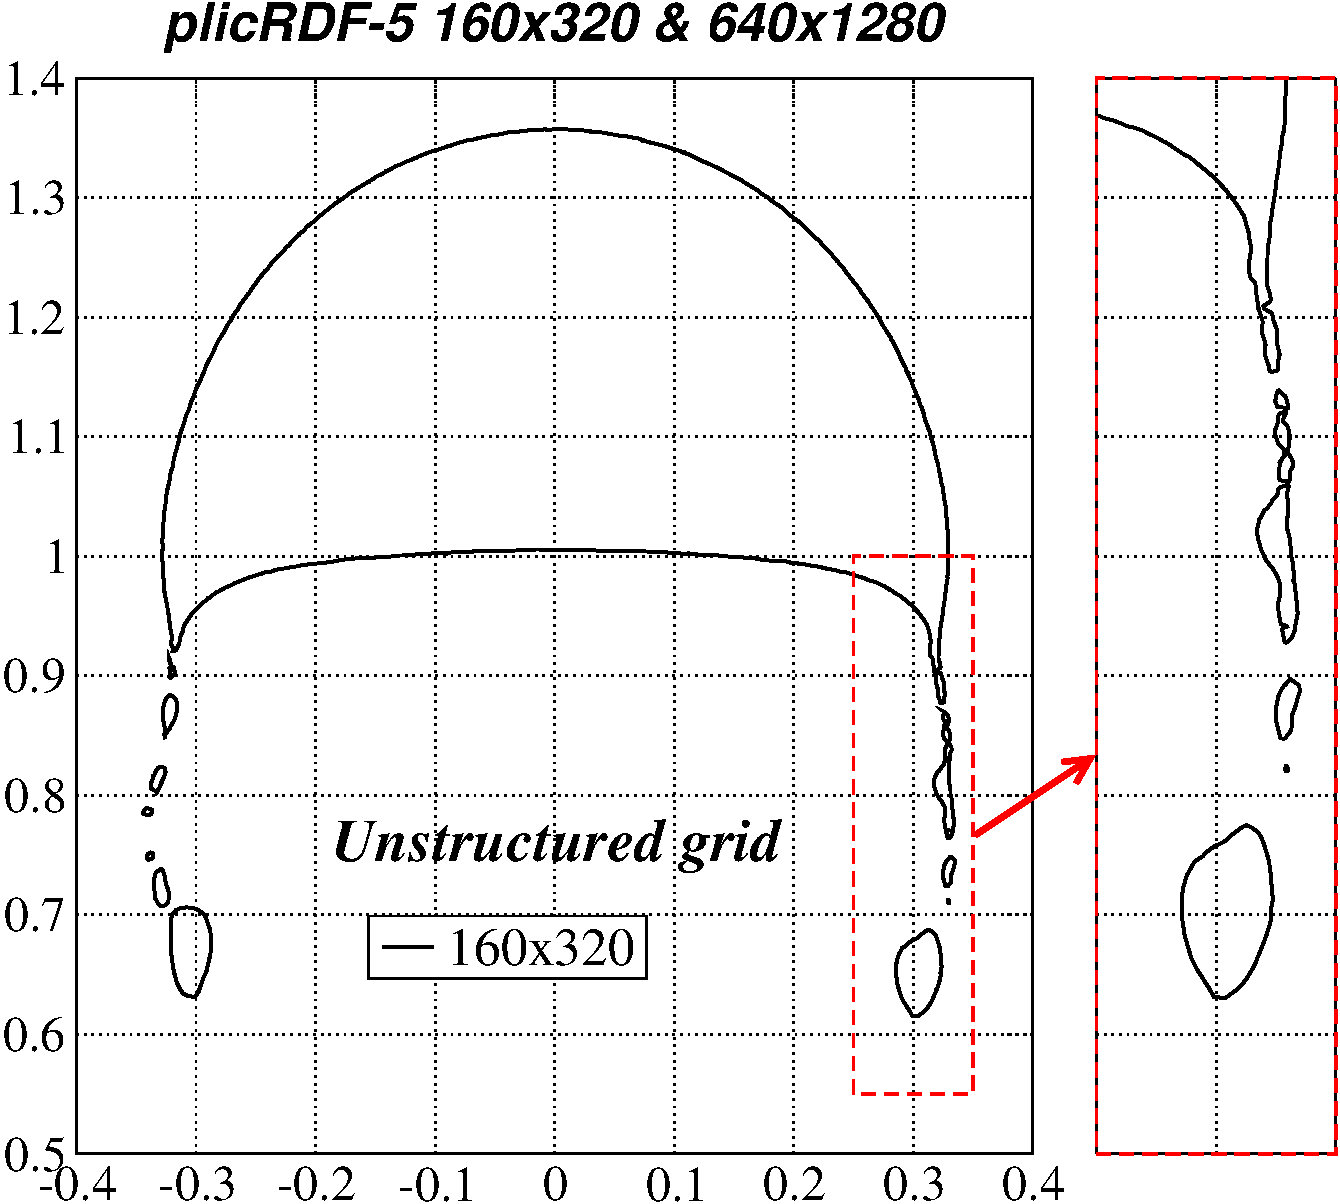
\includegraphics[width=0.45\textwidth]{figures/bubble_shape_t=3_plicRDF5-uns.pdf}
 \vspace{-6mm}
\end{center}
\caption{Bubble shape at time t=3 for isoAdvector plicRDF-5. Left: square grids, Right: triangular.}
\label{fig:HB_bubble_shape_3_plicRDF5}
\end{figure}


\begin{figure}[!h]
  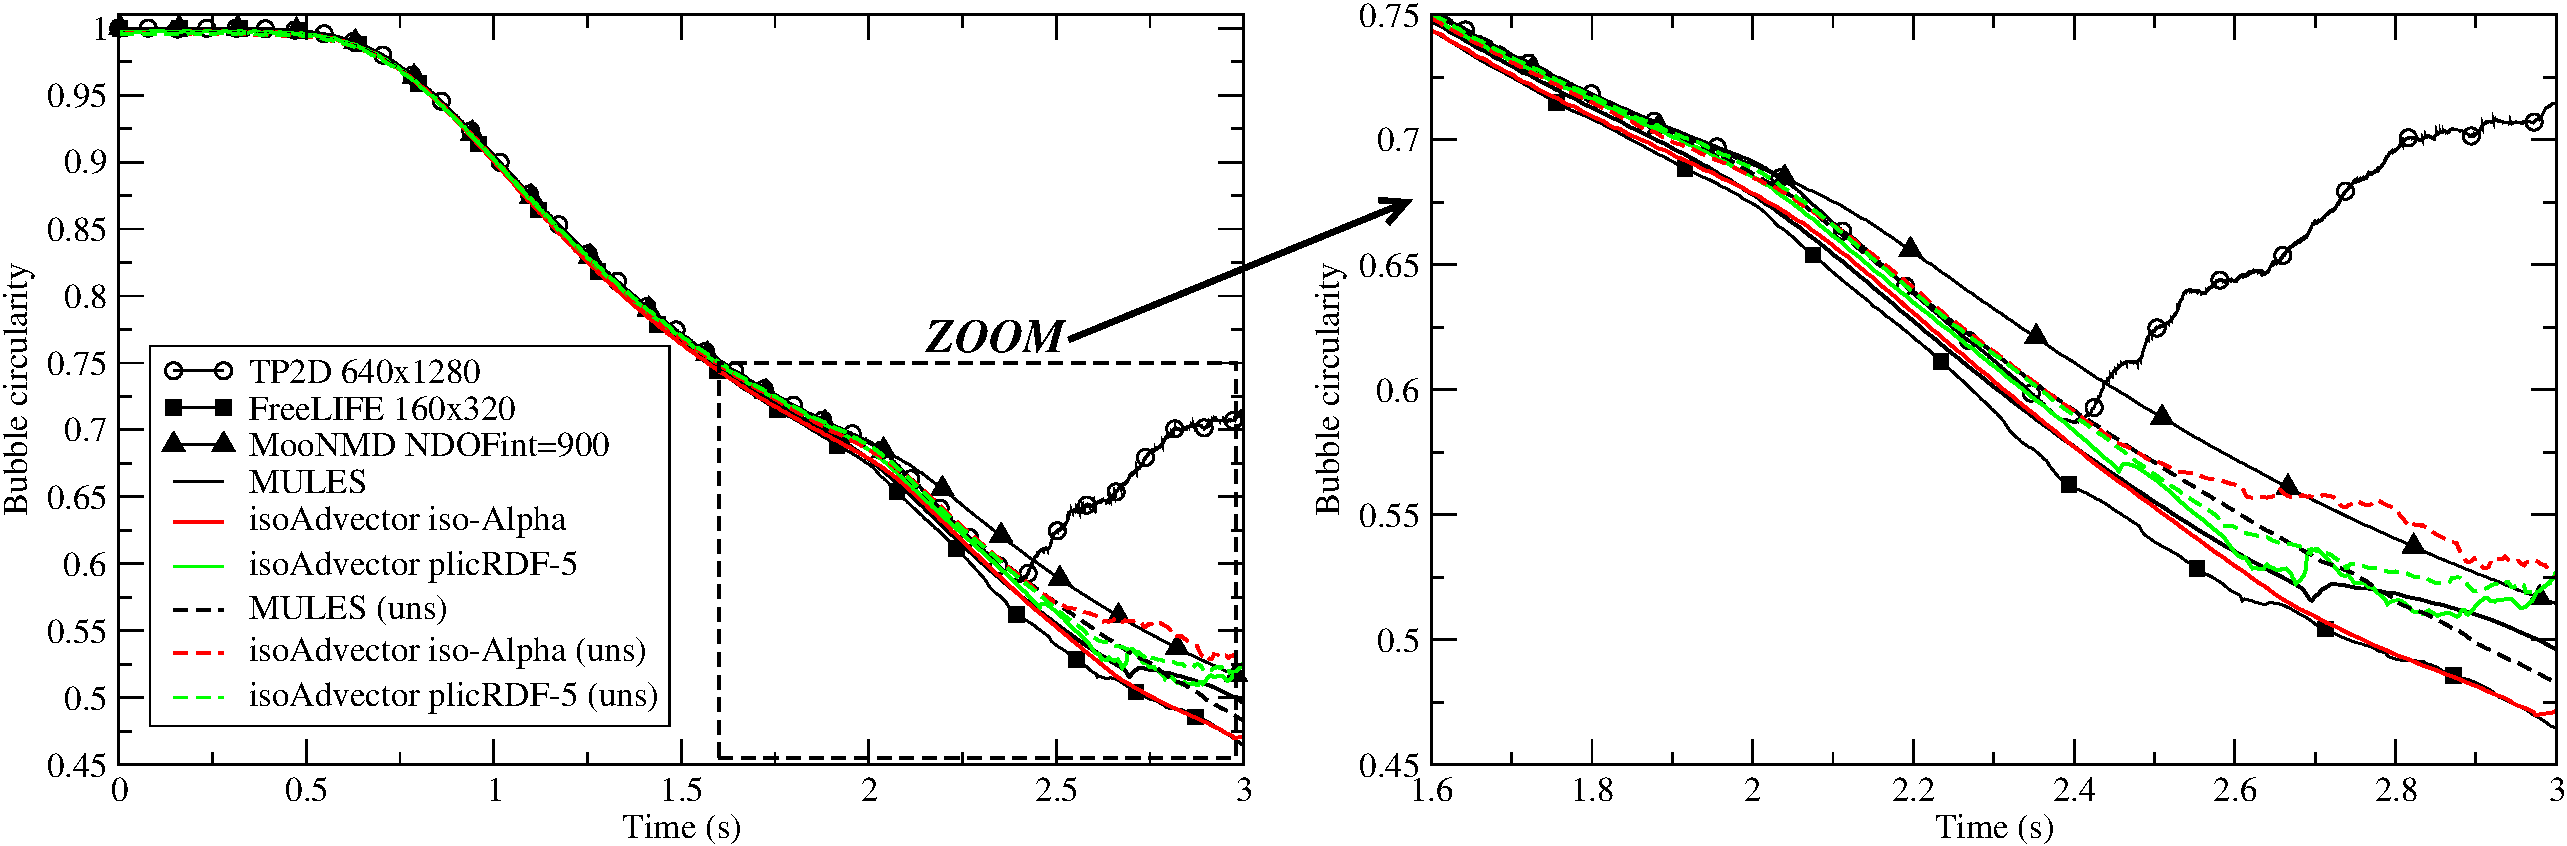
\includegraphics[width=\textwidth]{figures/HysingB_bubble_circularity_160x320.pdf}
  \caption{Bubble circularity at resolution $160\times320$. Comparison of MULES, isoAdvector isoAlpha and plicRDF-5 with reference data for both Cartesian and triangular grids.}
  \label{fig:HB_bubble_circularity160}
\end{figure}

\begin{figure}[!h]
  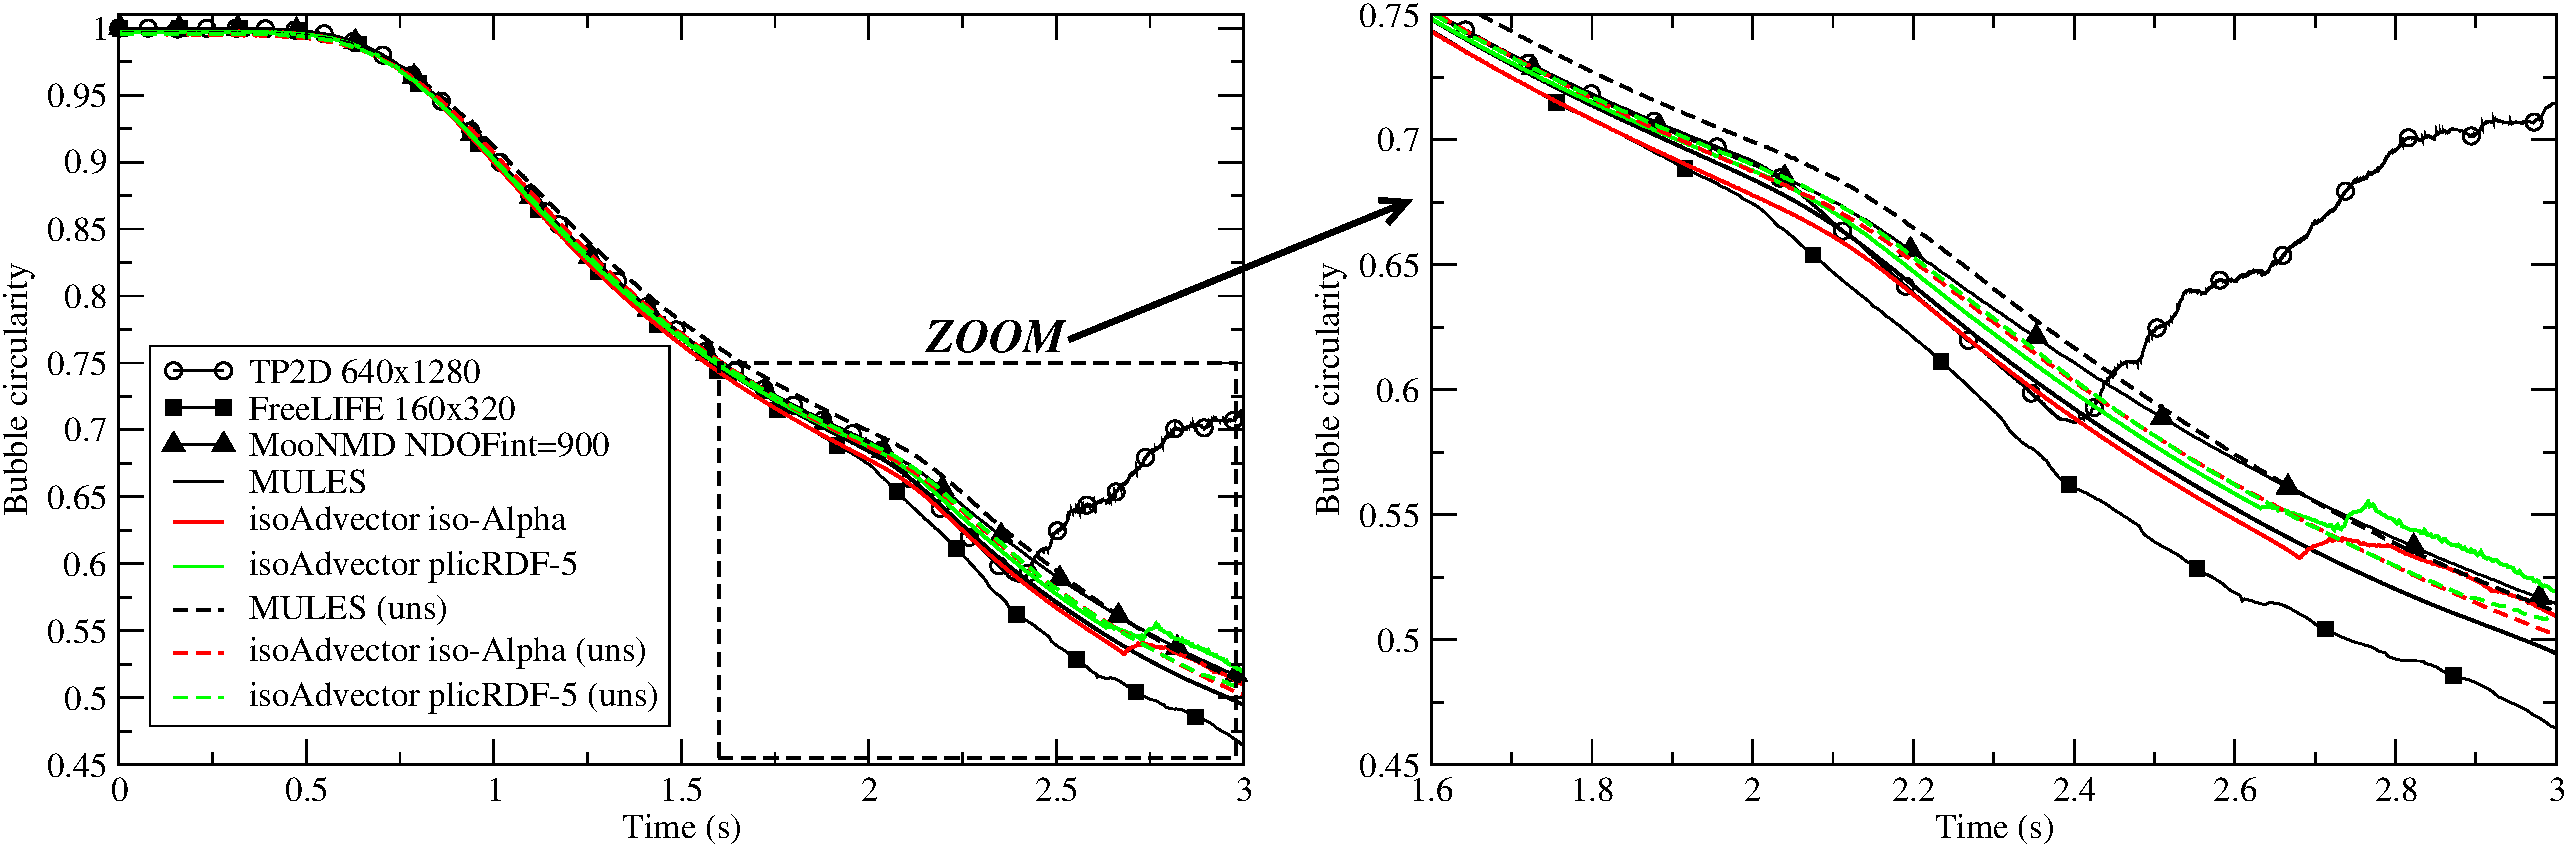
\includegraphics[width=\textwidth]{figures/HysingB_bubble_circularity_640x1280.pdf}
  \caption{Bubble circularity at resolution $640\times1280$. Comparison of MULES, isoAdvector isoAlpha and plicRDF-5 with reference data for both Cartesian and triangular grids.}
  \label{fig:HB_bubble_circularity640}
\end{figure}


\begin{figure}[!h]
  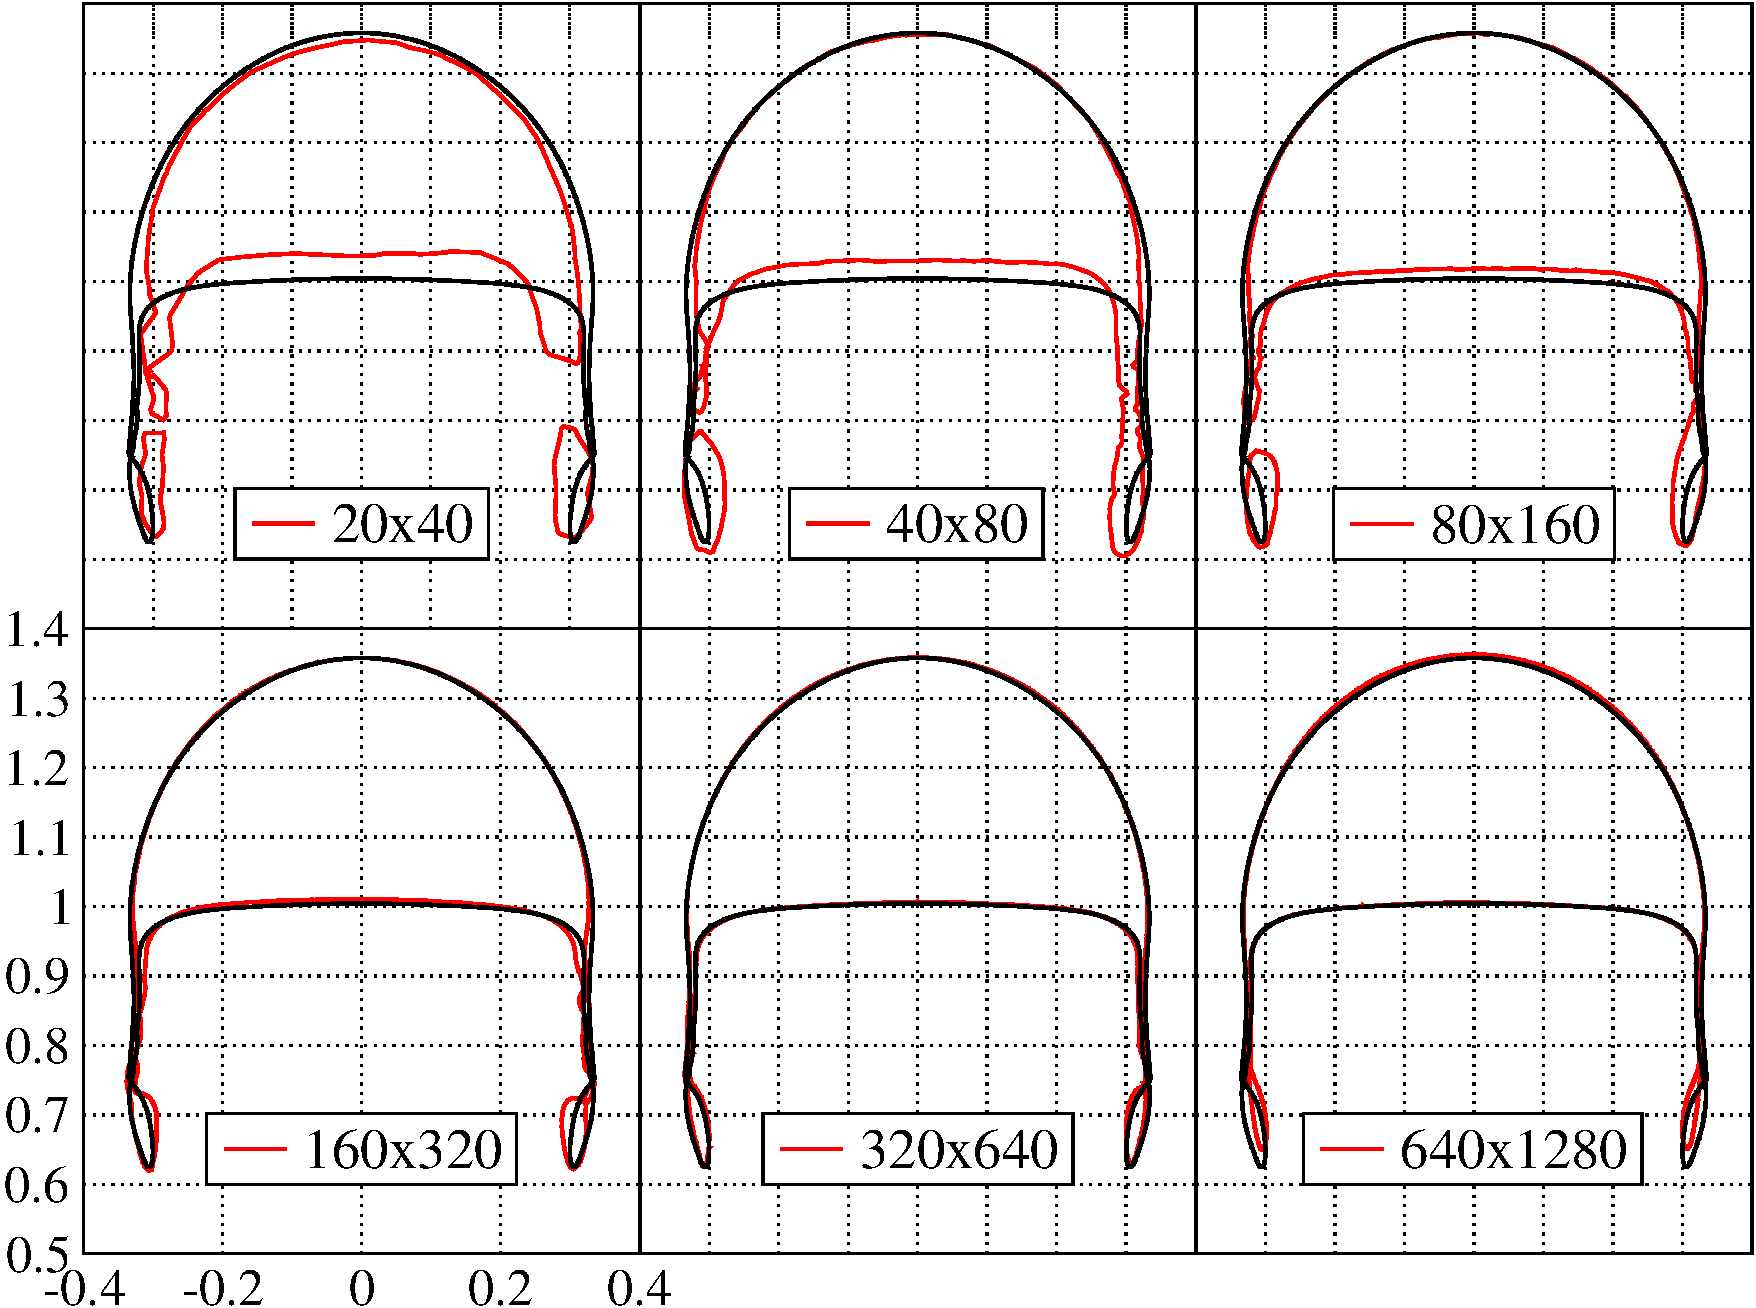
\includegraphics[width=\textwidth]{figures/bubble_shape_t=3_compareOFMULES_Fineststruct_vs_uns_grids.pdf}
  \caption{Comparison of bubble shape obtained on different resolution triangular grids (red) against the finest Cartesian grid at 640x1280 (black). Plots for MULES at time $t=3$.}
  \label{fig:HB_compareOFMULES_Fineststruct.vs.uns}
\end{figure}

\begin{figure}[!h]
  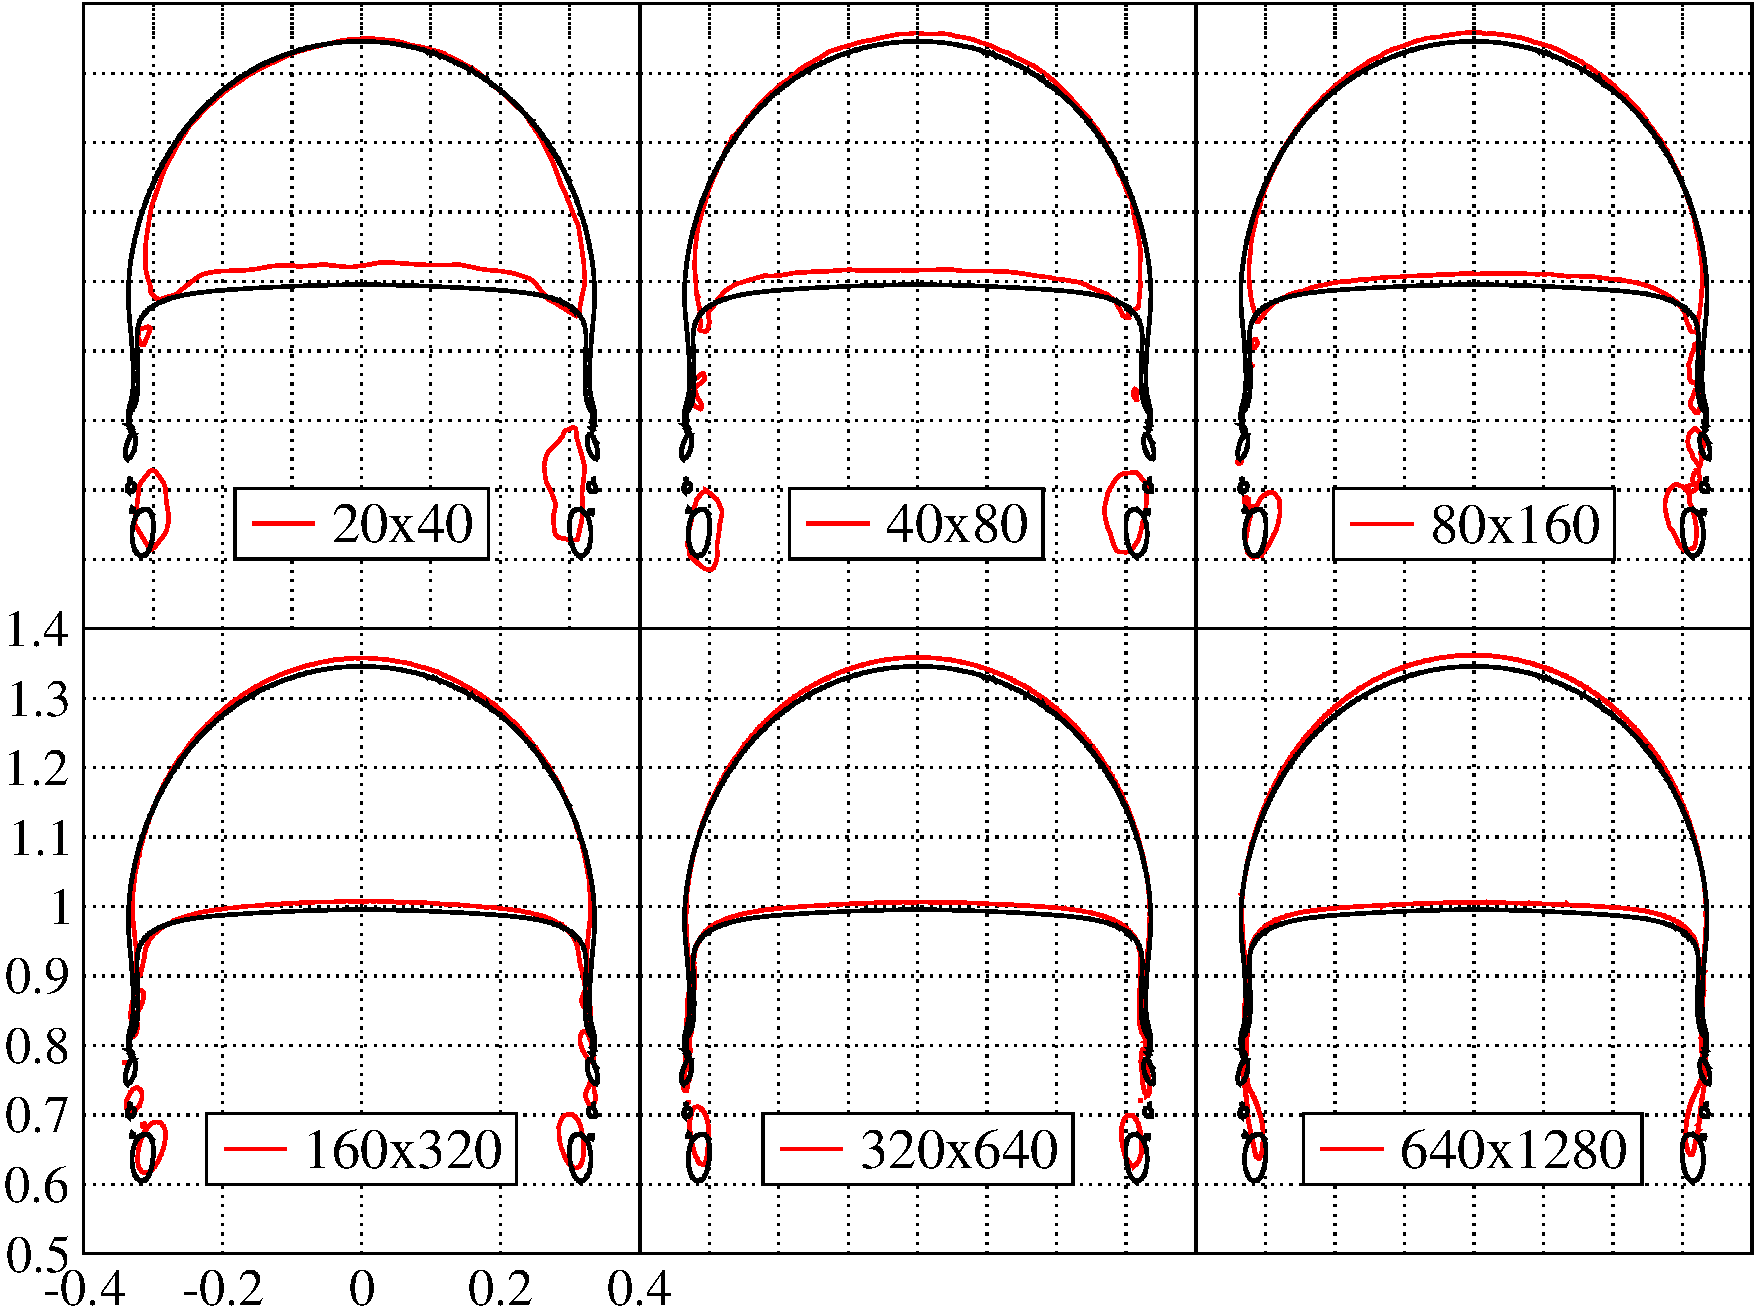
\includegraphics[width=\textwidth]{figures/bubble_shape_t=3_compareOFisoAlpha_Fineststruct_vs_uns_grids.pdf}
  \caption{Comparison of bubble shape obtained on different resolution triangular grids (red) against the finest Cartesian grid at 640x1280 (black). Plots for isoAdvector isoAlpha at time $t=3$.}
  \label{fig:HB_compareOFisoAlpha_Fineststruct.vs.uns}
\end{figure}

\begin{figure}[!h]
  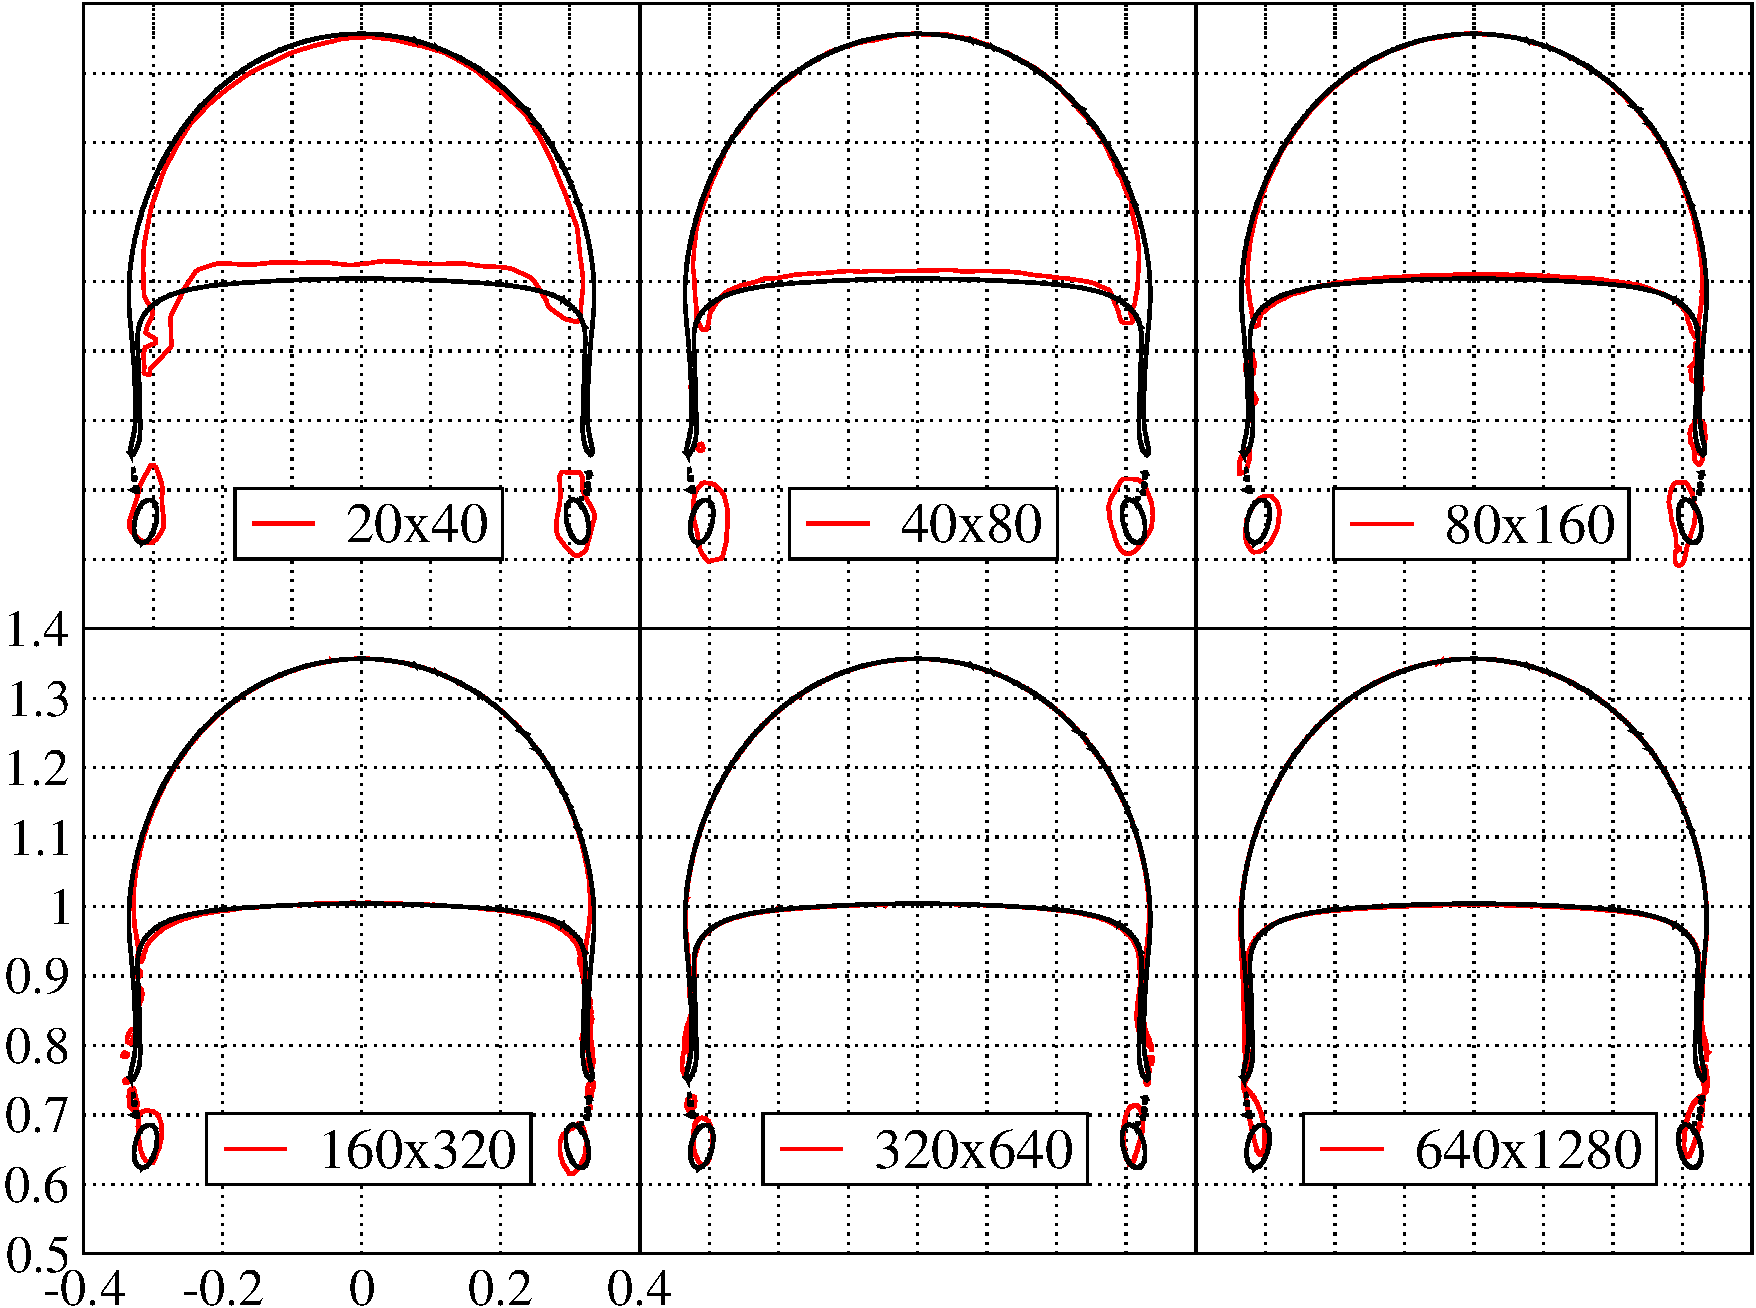
\includegraphics[width=\textwidth]{figures/bubble_shape_t=3_compareOFplicRDF5_Fineststruct_vs_uns_grids.pdf}
  \caption{Comparison of bubble shape obtained on different resolution triangular grids (red) against the finest Cartesian grid at 640x1280 (black). Plots for isoAdvector plicRDF-5 at time $t=3$.}
  \label{fig:HB_compareOFplicRDF5_Fineststruct.vs.uns}
\end{figure}

\begin{figure}[!h]
  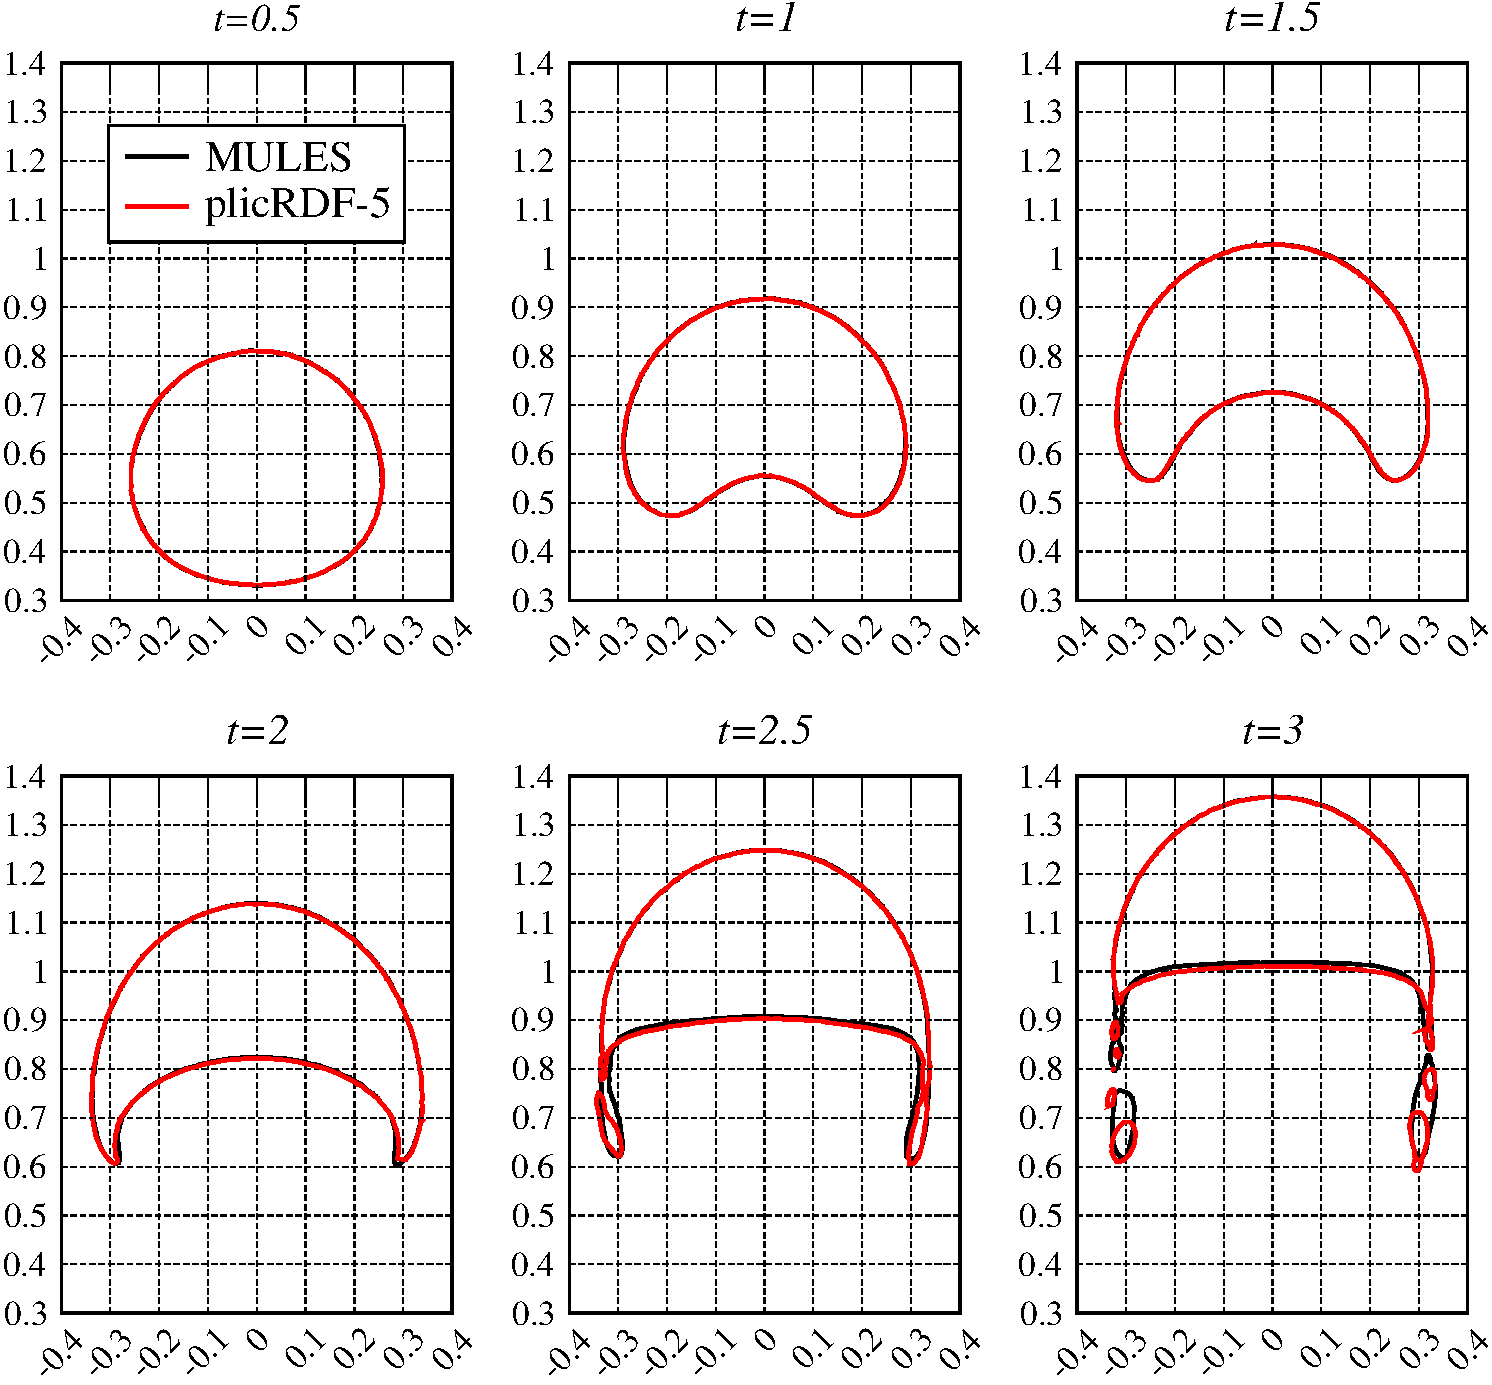
\includegraphics[width=\textwidth]{figures/bubble_shape_time_evol_uns080_MULES_vs_plicRDF5.pdf}
  \caption{Time sequence of bubble shape. Comparison of MULES with plicRDF-5 on a Cartesian grid of size 80x160.}
  \label{fig:HB_bubble_shape_time_evol_uns080_MULES_vs_plicRDF5}
\end{figure}

\begin{figure}[!h]
  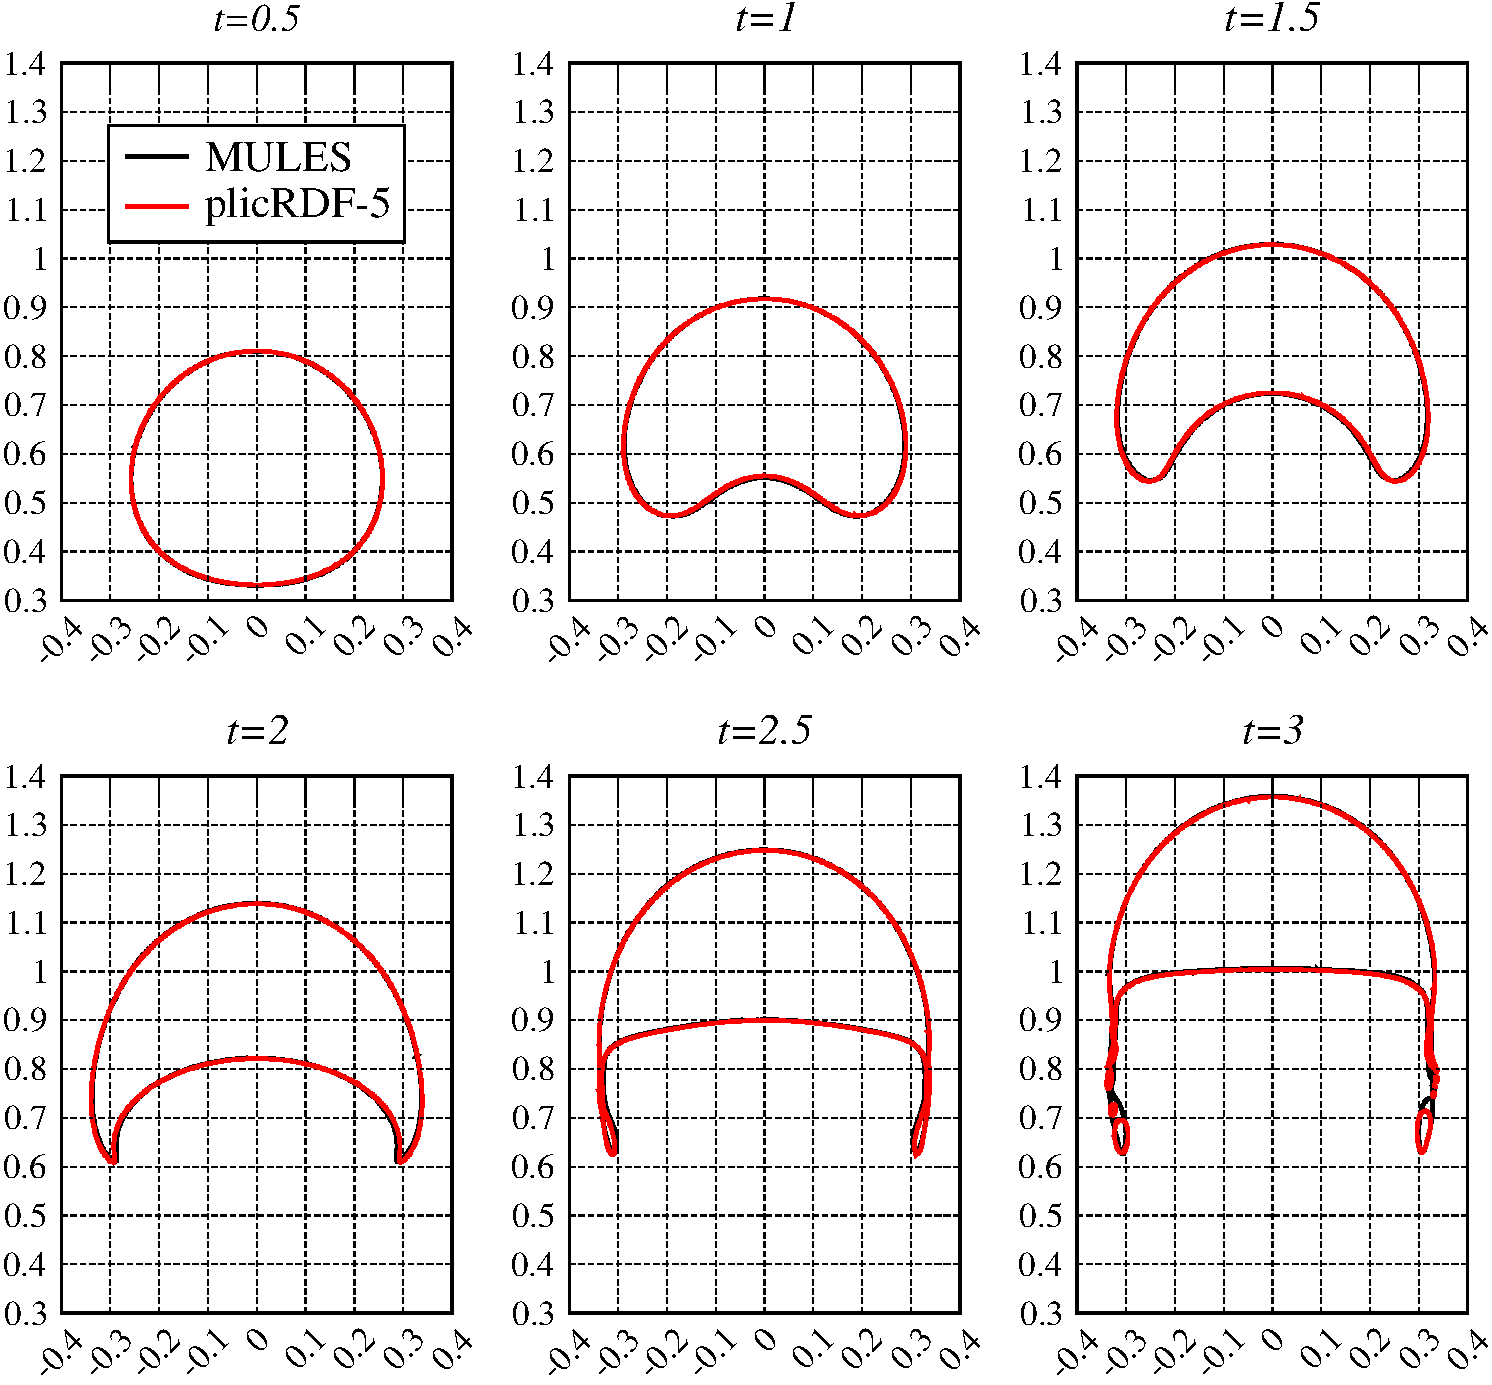
\includegraphics[width=\textwidth]{figures/bubble_shape_time_evol_uns320_MULES_vs_plicRDF5.pdf}
  \caption{Time sequence of bubble shape. Comparison of MULES with plicRDF-5 on a Cartesian grid of size 320x640.}
  \label{fig:HB_bubble_shape_time_evol_uns320_MULES_vs_plicRDF5}
\end{figure}




\clearpage
%%======================================================================
\section{Spurious currents quantification}\label{sec_spuriouscase}
%%======================================================================

In a static configuration such as the circular bubble studied in this section, the Navier-Stokes momentum equations~\ref{NSeqns} simplify to a balance between pressure gradient and volumic surface tension force. Spurious currents can occur from a numerical imbalance between the discretization of those two terms. This numerical imbalance creates a source term in the vorticity production equation, which in turn generates velocities. 
In an attempt to quantify the spurious currents generated by the OpenFOAM VoF methods studied here, this section uses a zero gravity single bubble test case, inspired from section~\ref{sec_hysingcase}. This elementary case provides a base of comparison of the OpenFOAM numerical methods with each other.

\subsection{Definition of test case}\label{sec_spuriouscasedef}
%%-----------------------------------------------------------------

As illustrated on figure~\ref{fig:spuriousCurrents_scheme}, we derived a zero gravity test case from the definition of the single rising bubble, stated in paragraph~\ref{sec_hysingcasedef}. The domain is now $1\times 1$ and the gravity is set to 0. All other physical and numerical parameters are kept identical. This test case is ideally not supposed to generate any velocity field. 

\begin{figure}[!h]
\begin{center}
 \vspace{-1mm}
 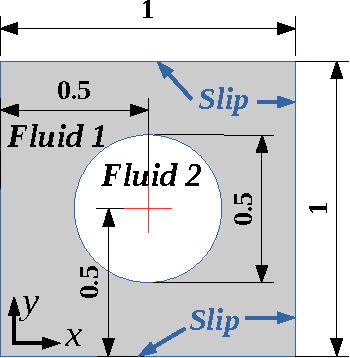
\includegraphics[width=4.25cm]{figures/spuriousCurrents_scheme.pdf}
 \vspace{-7mm}
\end{center}
\caption{Configuration and boundary conditions for 2D spurious currents test case.}
\label{fig:spuriousCurrents_scheme}
\end{figure}

\subsection{Results and discussion}\label{sec_spuriousresults}
%%-----------------------------------------------------------------
Figure~\ref{fig:spuriousCurrents_velocityField} shows a qualitative view of the spurious currents generated by the different OpenFOAM solvers used here. Note that plicRDF-5 vectors have been scaled by a factor 80 with respect to other solvers to make them visible.

In order to quantify these generated spurious velocities, we monitored the maximum of velocity magnitude over the computational domain. The result is shown on figures~\ref{fig:spuriousCurrents_MaxmagU_struct} and~\ref{fig:spuriousCurrents_MaxmagU_uns}, for, respectively, hexahedral and triangular grids. The same scales have been used on both plots. The noticeable point is that plicRDF-5 generates spurious vectors on hexahedral grids by almost two orders of magnitude smaller than other solvers, as shown on figure~\ref{fig:spuriousCurrents_MaxmagU_struct}. On hexahedral grids, MULES and isoAlpha velocity errors are not always lower for higher grid resolutions. On the other side, plicRDF-5 obtained reduced errors for higher grid resolutions. Compared to hexahedral grids, triangular grids generate more errors for all solvers (see figure~\ref{fig:spuriousCurrents_MaxmagU_uns}). isoAlpha errors increase with grid resolution, while MULES generates larger or equal errors. On triangular grids, plicRDF-5 generates spurious vectors by more than one order of magnitude smaller than other solvers, except for the highest resolution plotted (320x640 blue curve) where point-to-point oscillations occur on the maximum of velocity magnitude. 

Spurious velocities can have an influence on the shape of the bubble. In the present case with zero gravity, the bubble should remain 2D cylindrical. The graph of figure~\ref{fig:spuriousCurrents_bubble_error_radius_struct} (resp.~\ref{fig:spuriousCurrents_bubble_error_radius_uns}) shows the relative error on the radius in percent on hexahedral (resp. triangular) grids of increasing sizes. $r_0$ denotes the bubble radius at time $t=0$. For hexahedral grids, MULES and isoAlpha show maximal errors along the coordinate axes directions (at $0$, $\pm 90$ or $\pm 180$ degrees) and also along grid median directions at $45$ degrees. isoAlpha shows an increasing error when the grid resolution increases. plicRDF-5 errors are smaller, particularly along the coordinate axes directions. For triangular grids, errors displayed on figure~\ref{fig:spuriousCurrents_bubble_error_radius_uns} no longer show preferential directions. They are also larger than on figure~\ref{fig:spuriousCurrents_bubble_error_radius_struct}. Like for hexahedral grids, plicRDF-5 errors are also reduced with respect to other OpenFOAM solvers. 

Finally, the plot of figure~\ref{fig:spuriousCurrents_pressure_jump} shows the pressure jump across the middle of the bubble along the horizontal direction~$x$. The Young-Laplace law for the pressure discontinuity due to surface tension can be expressed as:
\begin{equation}
  \Delta p = \sigma \, \left( \frac{1}{R_1} + \frac{1}{R_2} \right)
  \label{eqnYoungLaplace}
\end{equation}
where $R_1$ and $R_2$ are curvature radii along two perpendicular directions. As the present case involves a 2D cylindrical bubble which is infinite in the~$z$ direction, one of the curvature radius can thus be taken as infinite. The second curvature radius in the perpendicular direction is the bubble radius, which can be approximated as the initial bubble radius $r_0=0.25$m. The pressure jump across the bubble can so be computed as $\Delta p=7.84$Pa. This theoretical solution is plotted as the dashed green line in figure~\ref{fig:spuriousCurrents_pressure_jump}. Both for hexahedral and triangular grids, plicRDF-5 provides the best fit to the theoretical rectangular function of pressure jump across this bubble under 0 gravity. MULES and isoAlpha solvers conduct to underestimated pressure in the gas region, presenting over or undershoot near the pressure discontinuities at the fluids interface.

\begin{figure}[!h]
 \begin{center}
   \vspace{-1mm}
   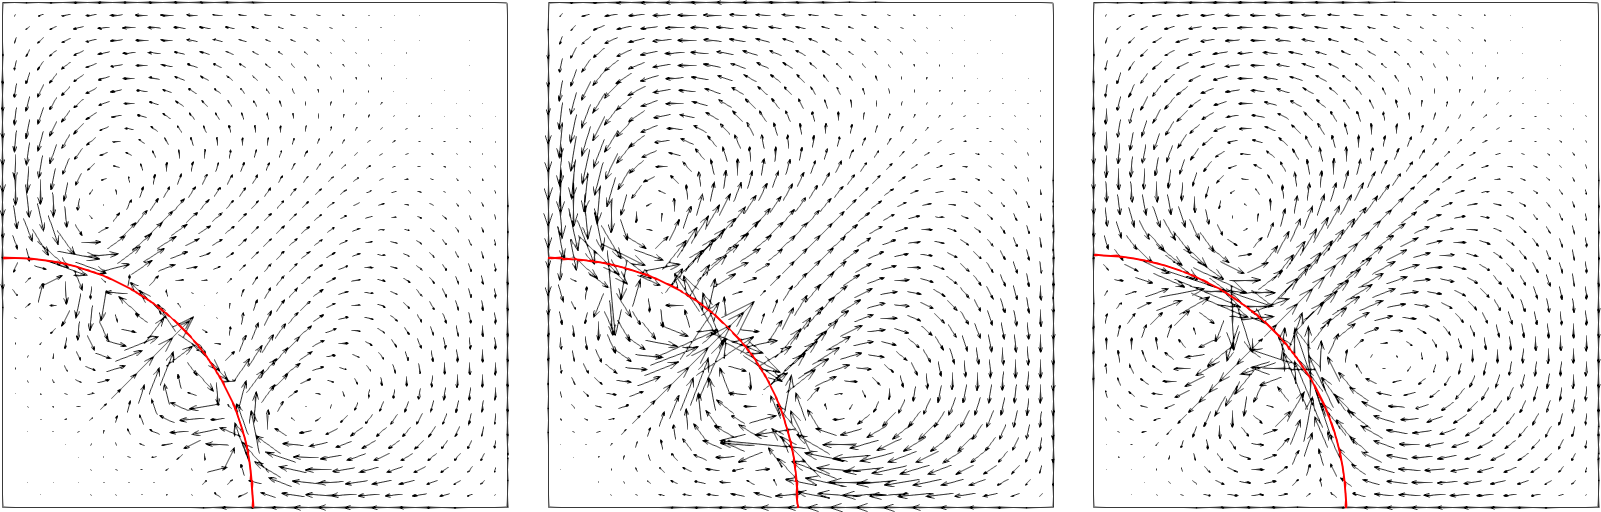
\includegraphics[width=\textwidth]{figures/spuriousCurrents_MULES_vs_isoAlpha_vs_plicRDF-5-scaleX80_time=1p5_080x160_quarter.png}
 \end{center}
 \vspace{-11mm}
 \begin{tabular}{p{0.3\textwidth}p{0.3\textwidth}p{0.3\textwidth}}
    \begin{center}
    $\mathbf{scale \times 1}$
    \end{center} 
    & 
    \begin{center}
    $\mathbf{scale \times 1}$ 
    \end{center} 
    & 
    \begin{center}
    $\mathbf{scale \times 80}$
    \end{center}
    \\
 \end{tabular}
 \vspace{-11mm}
\caption{Bubble under 0 gravity: Visualization of spurious currents at time $t=1.5$ in top right quarter. Left: MULES. Middle: isoAlpha. Right: plicRDF-5. Vectors on the r.h.s. plicRDF-5 image are scaled by a factor 80 with respect to MULES or isoAlpha. The red line materializes the isoline $\alpha=0.5$.}
\label{fig:spuriousCurrents_velocityField}
\end{figure}

\begin{figure}[!h]
  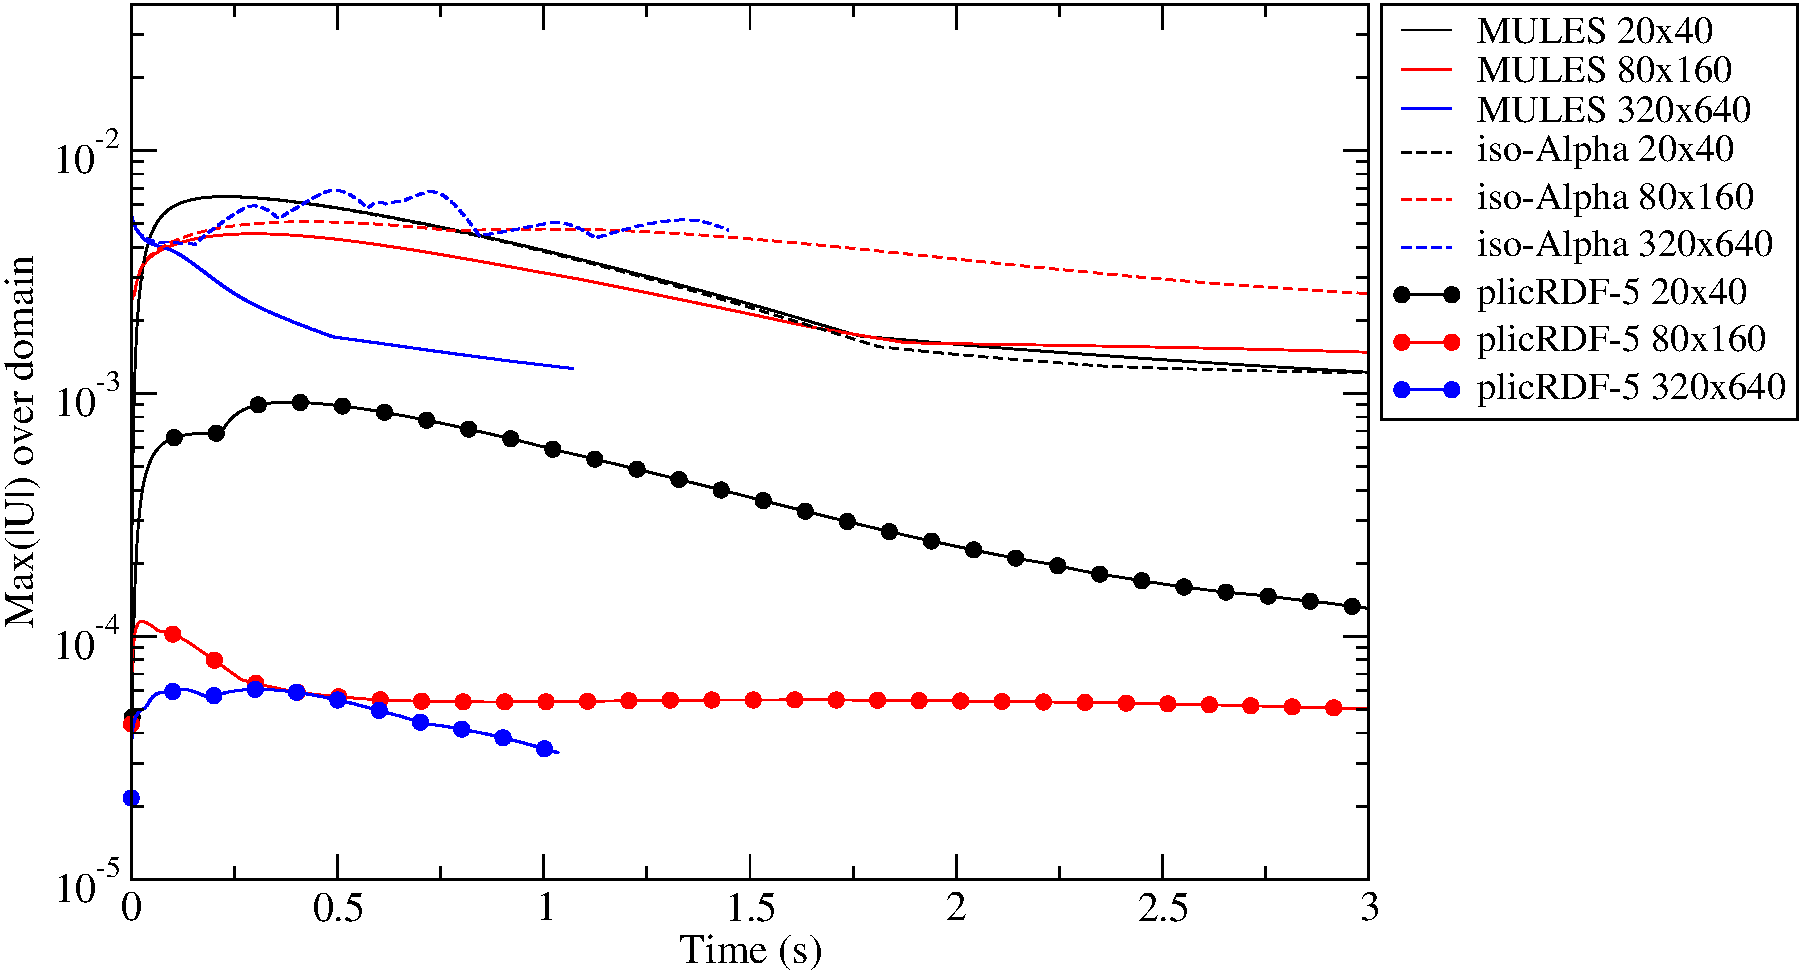
\includegraphics[width=\textwidth]{figures/spuriousCurrents_MaxmagU_compareOF_20_80_320_struct.pdf}
  \caption{Bubble under 0 gravity: Maximum magnitude of spurious velocities over the computational domain for hexahedral grids.}
  \label{fig:spuriousCurrents_MaxmagU_struct}
\end{figure}

\begin{figure}[!h]
  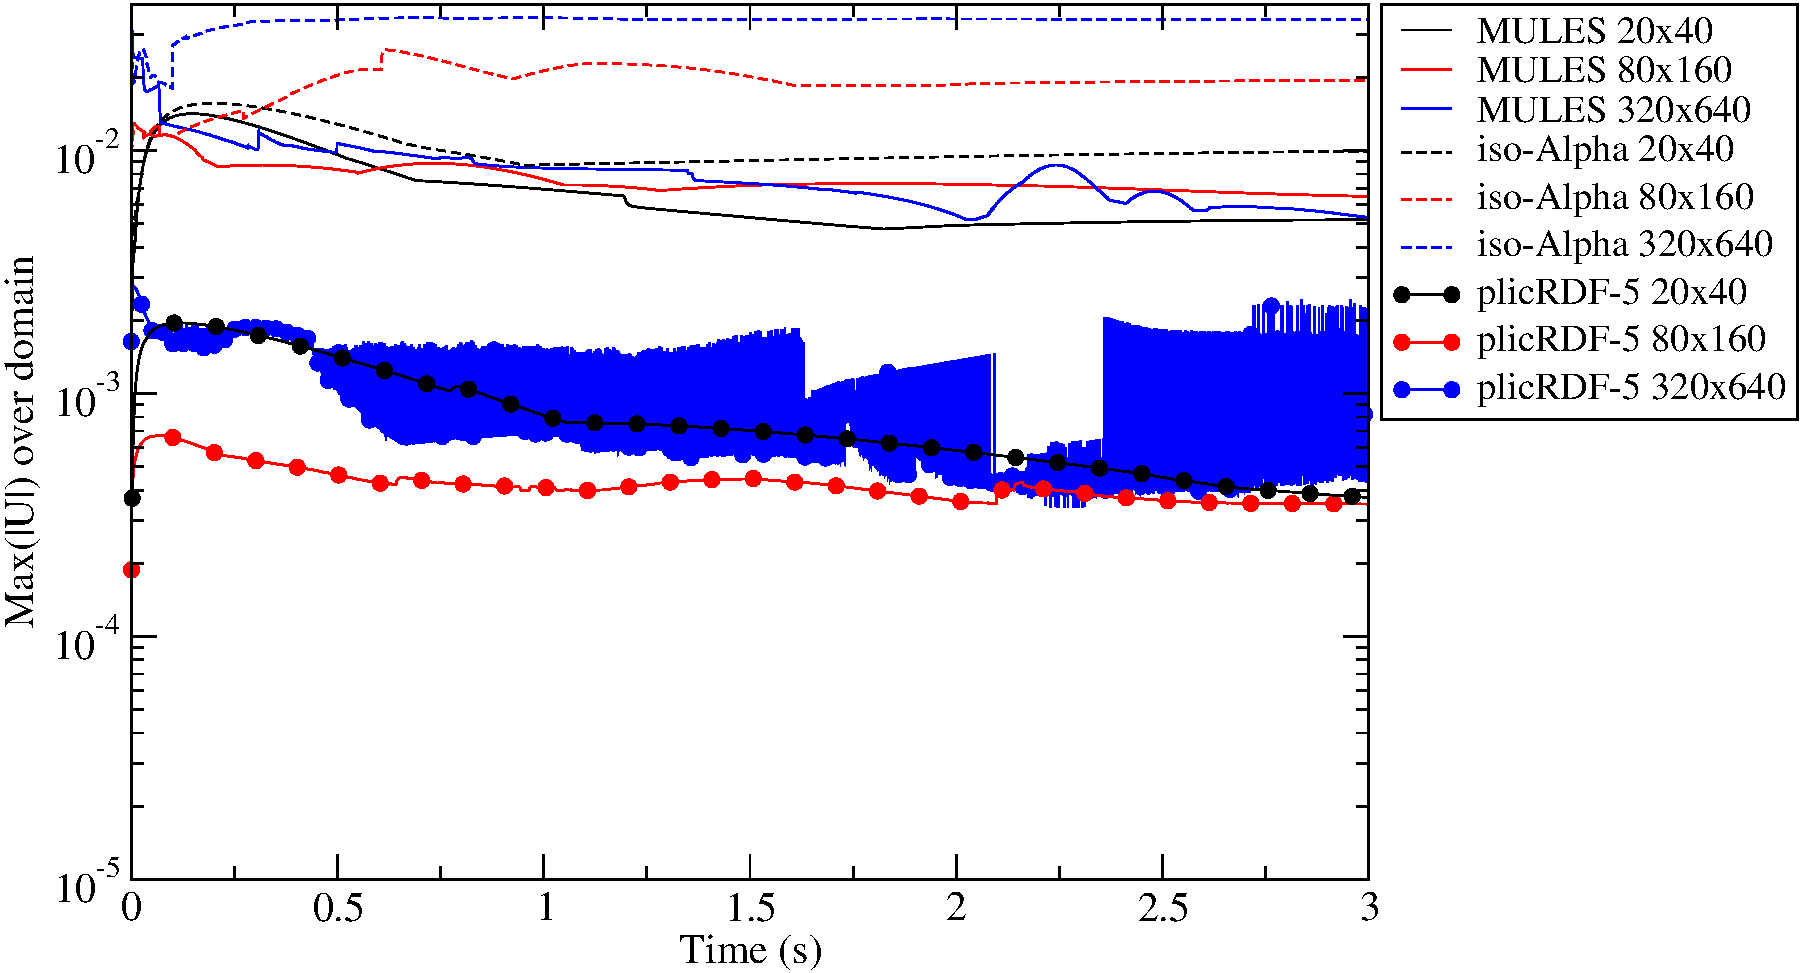
\includegraphics[width=\textwidth]{figures/spuriousCurrents_MaxmagU_compareOF_20_80_320_uns.pdf}
  \caption{Bubble under 0 gravity: Maximum magnitude of spurious velocities over the computational domain for triangular grids.}
  \label{fig:spuriousCurrents_MaxmagU_uns}
\end{figure}

\begin{figure}[!h]
  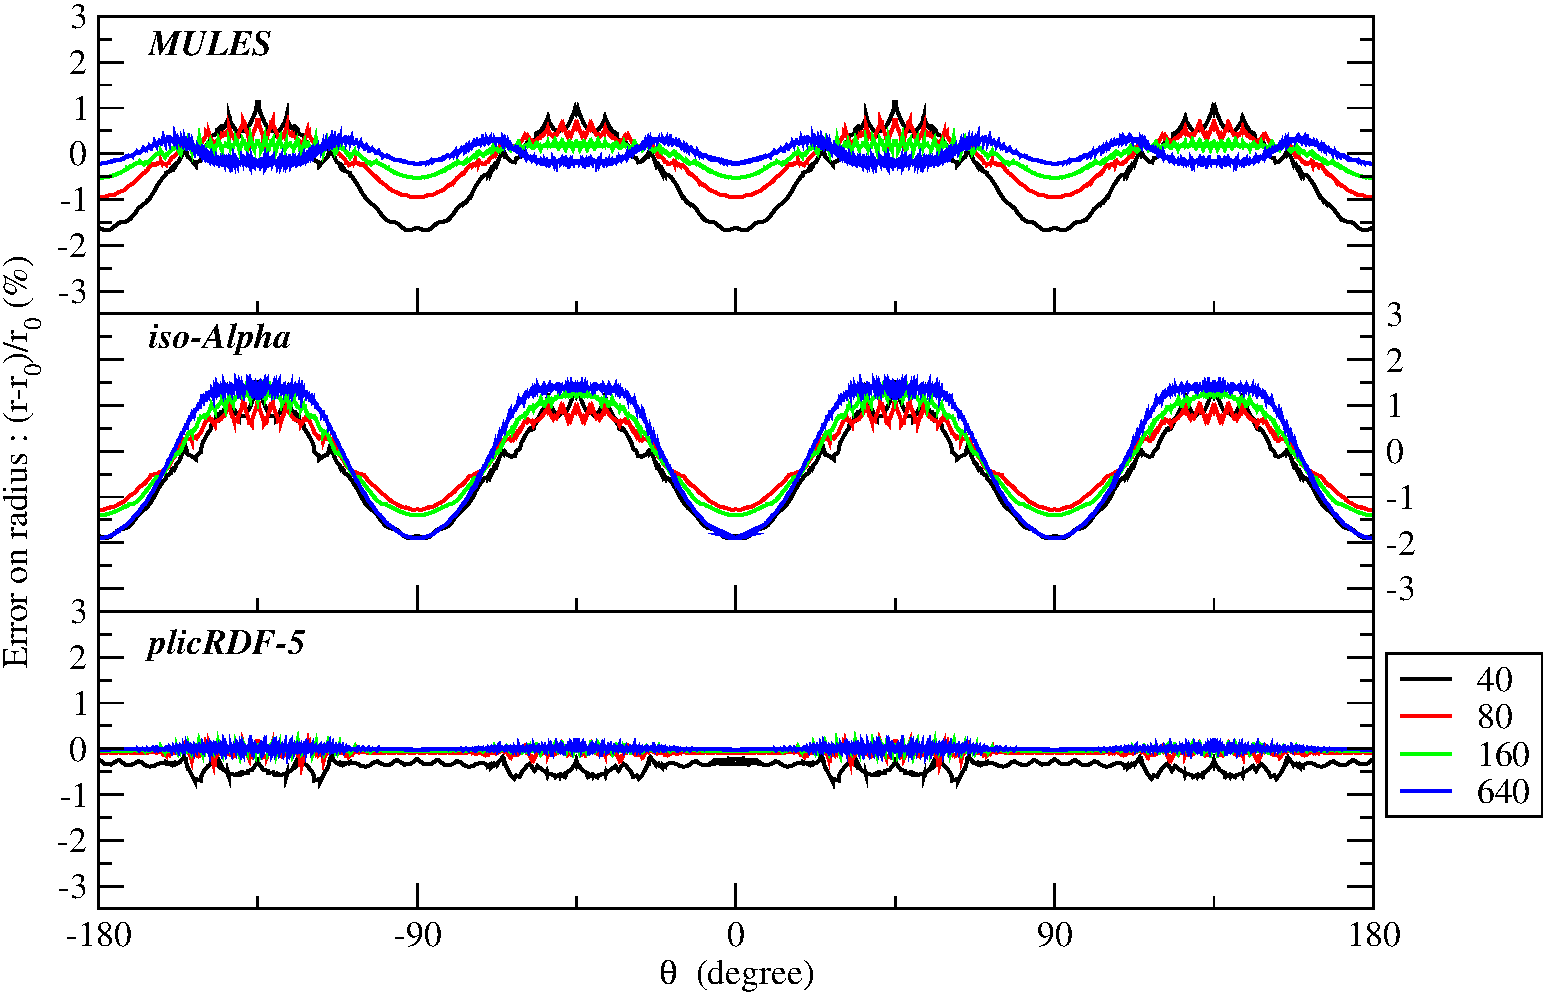
\includegraphics[width=\textwidth]{figures/spuriousCurrents_bubble_error_radius_struct.pdf}
  \caption{Bubble under 0 gravity: Error on bubble radius for hexahedral grids.}
  \label{fig:spuriousCurrents_bubble_error_radius_struct}
\end{figure}

\begin{figure}[!h]
  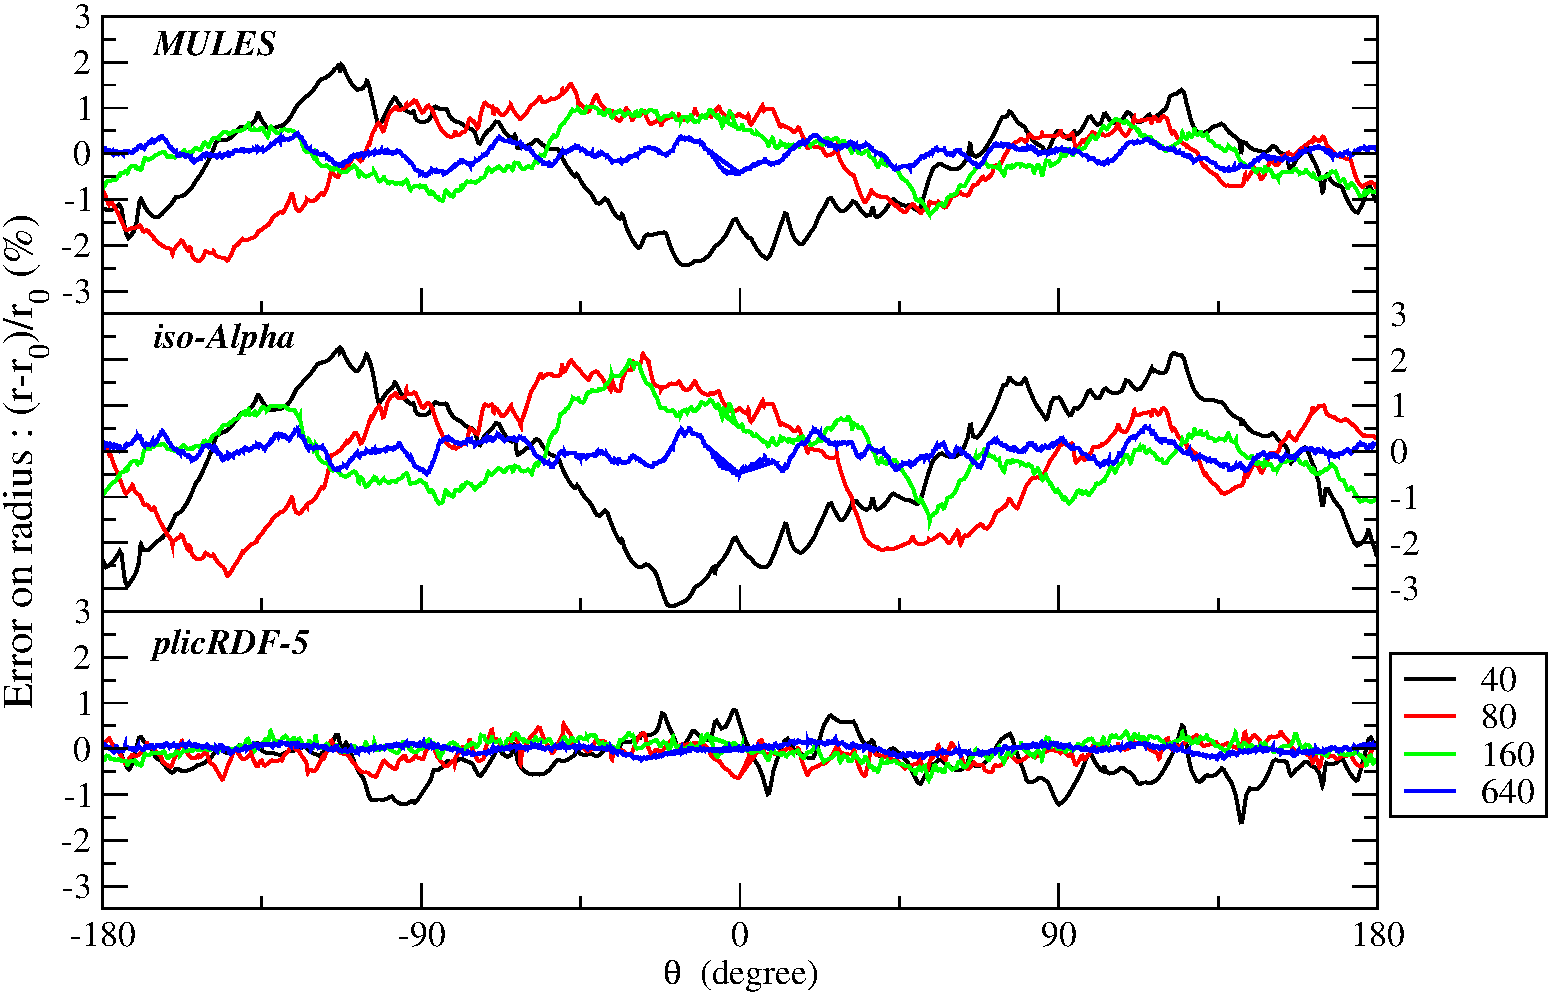
\includegraphics[width=\textwidth]{figures/spuriousCurrents_bubble_error_radius_uns.pdf}
  \caption{Bubble under 0 gravity: Error on bubble radius for triangular grids.}
  \label{fig:spuriousCurrents_bubble_error_radius_uns}
\end{figure}

\begin{figure}[!h]
  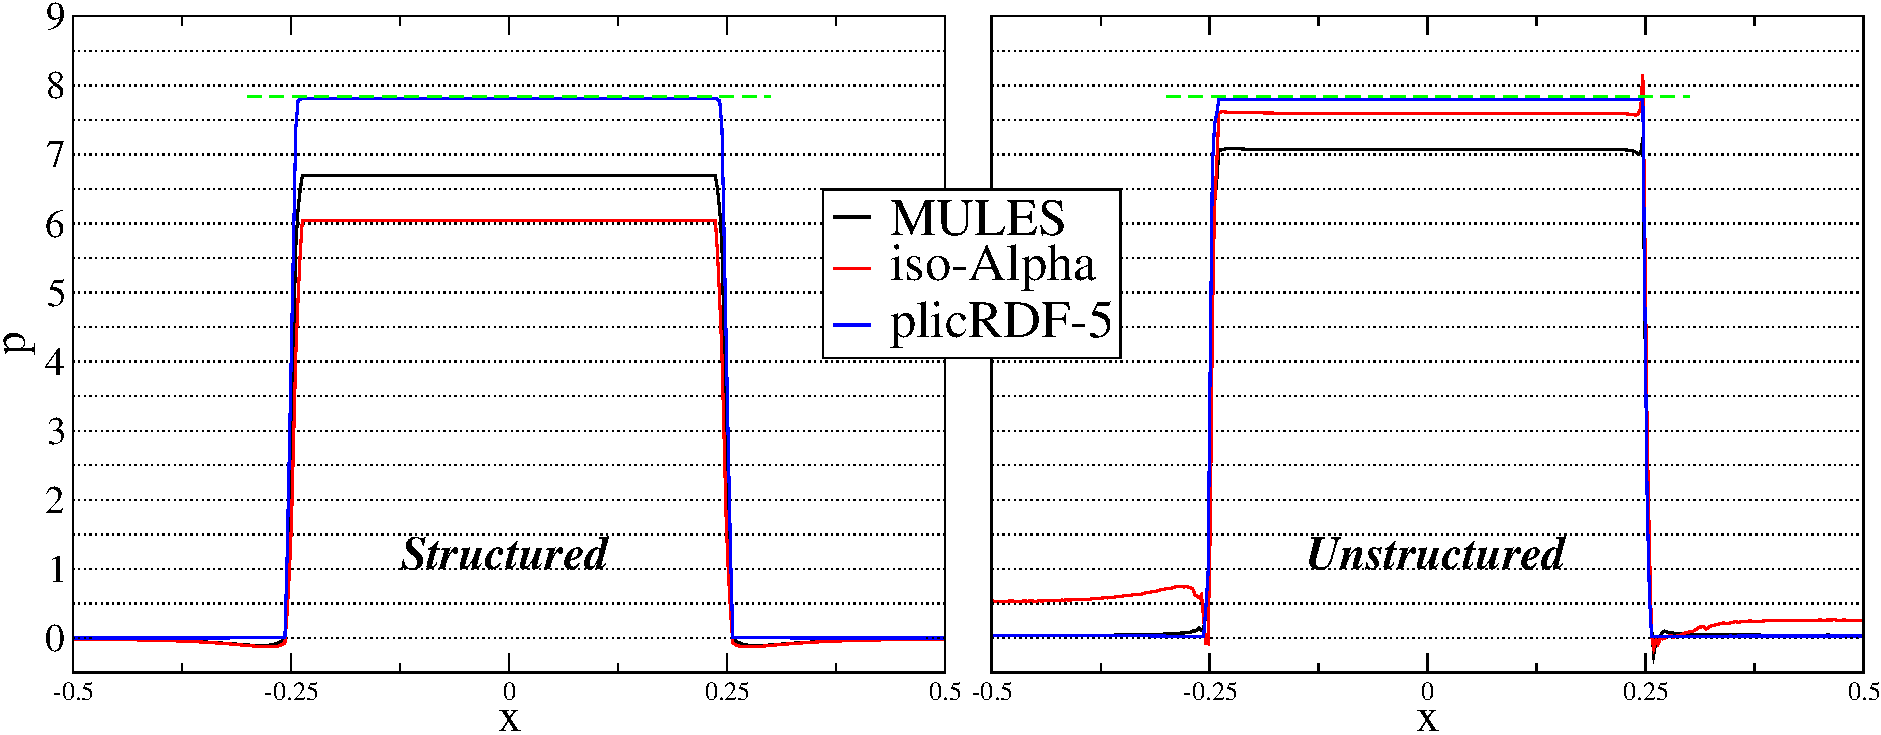
\includegraphics[width=\textwidth]{figures/spuriousCurrents_pressure_drop_t=3_160x320.pdf}
  \caption{Bubble under 0 gravity: Pressure jump across the bubble at time $t=3$.}
  \label{fig:spuriousCurrents_pressure_jump}
\end{figure}



%%======================================================================
\section{\small Conclusion}
%%======================================================================

We have presented a quantitative validation of the isoAdvector method (isoAlpha and plicRDF-5) against MULES and other solvers from reference data in the literature. Two 2D test cases have been used. The first test case is the Hysing benchmark, as originally published by Hysing~\cite{Hysing2009}. This benchmark simulates a single bubble rising in a initially quiescent liquid. isoAdvector has been verified to work for rising bubble simulation with similar or greater accuracy as MULES and with a sharper interface and slightly smaller calculation times. These results demonstrate that isoAdvector can be used for surface tension dominated flows. However, the sharper interface poses a challenge to the surface tension model in some simulations, for example at high resolutions or on unstructured triangular-prisms grids. The new reconstruction method, plicRDF-5, rectifies these problems. The second validation case presented in this study aims at quantifying the spurious currents obtained in the three VoF variants tested here (MULES, isoAlpha and plicRDF-5). This second configuration consists in a 2D stagnant single bubble in a quiescent liquid, under zero gravity conditions. The case has been derived from the rising bubble benchmark, using similar physical and numerical parameters, except gravity and fluid domain size. The new reconstruction method, plicRDF-5, significantly reduces the spurious currents due to its more accurate interface curvature calculation. Moreover, the plicRDF-5 reconstruction method demonstrates a better prediction of the pressure jump across the bubble. 


%%======================================================================
\section*{Acknowledgments}
%%======================================================================
\noindent
This  work  was  granted  access  to  the  HPC  resources  of CINES under the 
allocation 2018-AP012B10362 made by GENCI.

\clearpage
%%======================================================================
\section*{References}
%%======================================================================

\bibliography{references.bib}

\end{document}
